
\RequirePackage[pdf]{layout/hp-book}










\begin{document}
{
\pagestyle{empty}
\def\volumenumber{}
\def\volumetitle{Kapitel 1--\ref{last:chapter}} %  plus omake files 1--{4}
\newcommand{\fullvolumetitle}{\volumetitle}

\def\volumenumber{}
% \def\volumetitle{Layout-Test vom \today{}}
\def\volumetitle{}
\definecolor{gold}{rgb}{0.77,0.69,0.37}
\newlength{\hptitlewidth}
\newlength{\rationalh}
\newcommand{\hptitle}[2][\stockwidth]{%
\setlength{\hptitlewidth}{#1}%
\centering\color{white}%
\vskip 3cm\resizebox{.95\hptitlewidth}{!}{\textls[100]{HARRY POTTER AND THE}}%
\vskip 2mm%
\color{gold}%
\settoheight{\rationalh}{\resizebox{.95\hptitlewidth}{!}{\textls[20]{RATIONALITY}}}
\resizebox{!}{0.9\rationalh}{\textls[50]{METHODS}}%
\hfil\resizebox{!}{0.3\rationalh}{\textls[50]{Of}}%
\vskip 2mm%
\resizebox{.95\hptitlewidth}{!}{\textls[20]{RATIONALITY}}%
\vskip 8mm%
\color{white}%
\resizebox{.5\hptitlewidth}{!}{\textls[50]{\scshape{}Fanfiction von Eliezer Yudkowsky}}%
\vskip 4mm%
\resizebox{.35\hptitlewidth}{!}{\textls[50]{\scshape{}Deutsche Übersetzung}}%
\vfill%
\textls[50]{\scshape #2}%
\color{black}%
\vskip 1cm\ %
}
\providecommand{\fullvolumetitle}[1]{Buch #1: \volumetitle}

\ifcover%
\definecolor{backgroundcover}{HTML}{272c36}
\newpagecolor{backgroundcover}\afterpage{\restorepagecolor}
\newcommand\BackgroundPic{
\put(0,0){%
\parbox[b][\paperheight]{\paperwidth}{%
\vfill%
\centering%
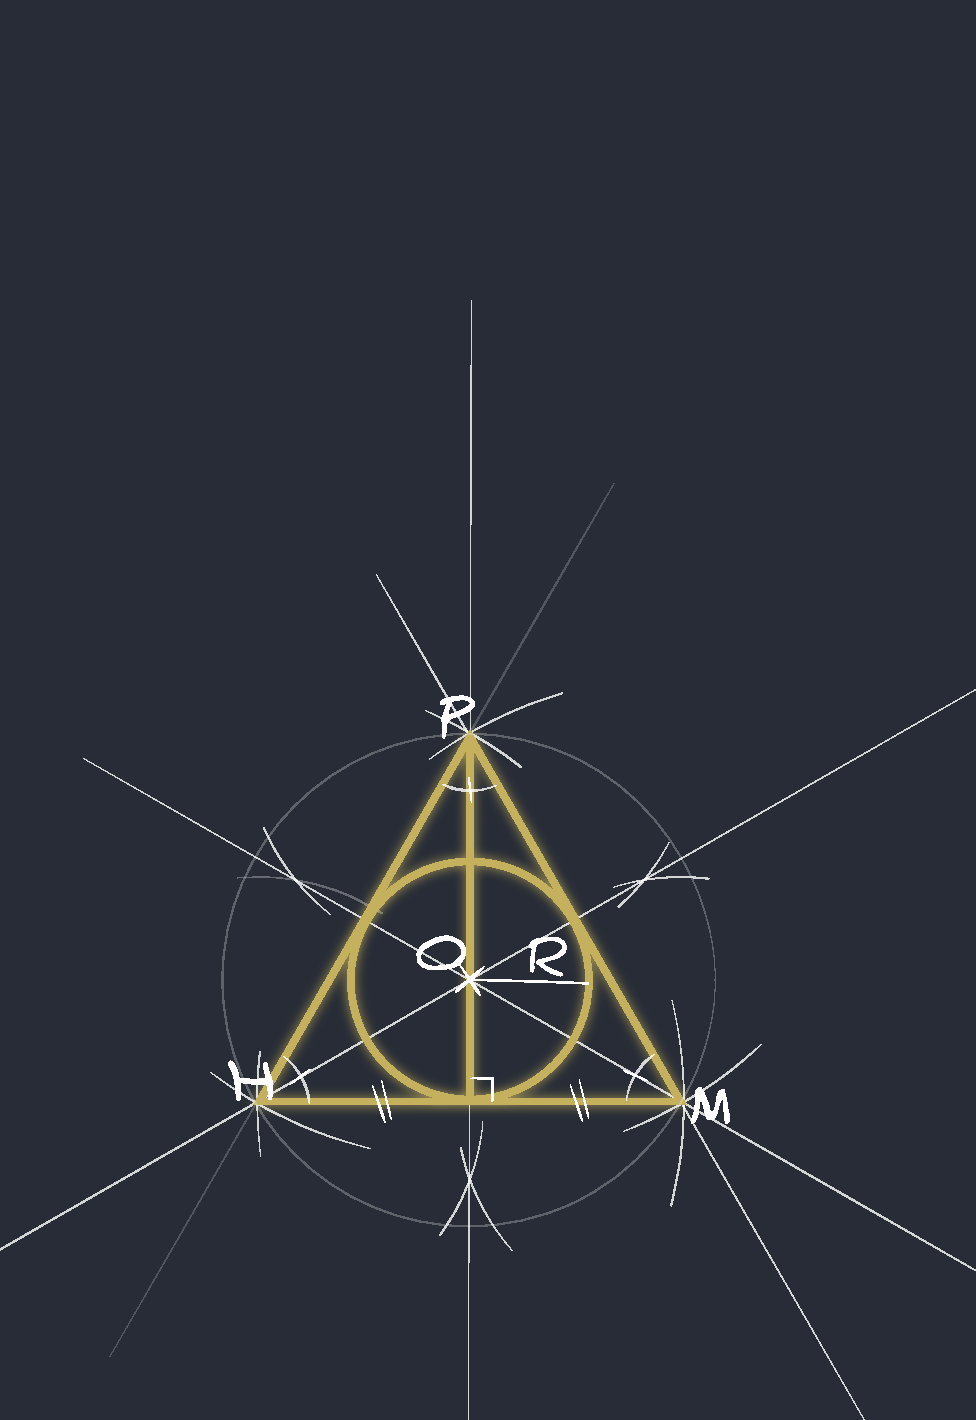
\includegraphics[width=\paperwidth,height=\paperheight,keepaspectratio]{images/cover1.pdf}%
\vfill%
}}}\AddToShipoutPicture*{\BackgroundPic}%
\AddToShipoutPicture*{\put(0,0){%
\parbox[b][\paperheight]{\paperwidth}{%
\hptitle{\fullvolumetitle{\volumenumber}}%
}}}%
\ %
\cleartorecto
\fi
\begin{center}
\thispagestyle{empty}
{\hpfont
\Huge\MakeUppercase{Harry Potter}\vspace*{0.5cm}

\Large\MakeUppercase{and the Methods of Rationality} %

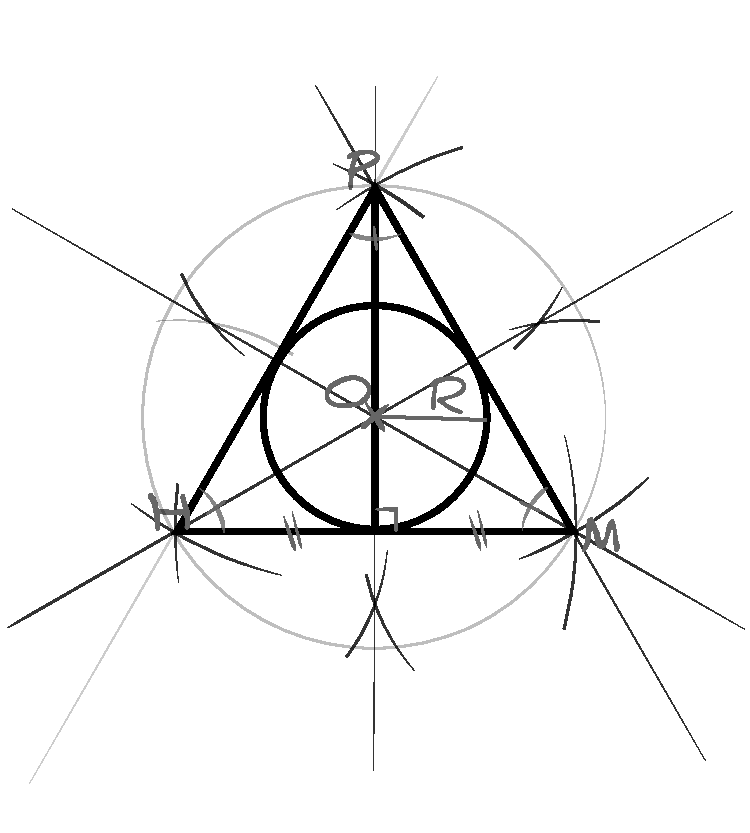
\includegraphics[scale=0.5]{images/bubble.pdf}

\vspace*{-1.0cm}
\Large Fanfiction von \vspace*{.25cm}

\huge \MakeUppercase{Eliezer Yudkowsky}%

\normalsize

\vspace*{1\baselineskip}
\fullvolumetitle{\volumenumber}
}

\vspace{0.7cm}

Basierend auf der Harry Potter Serie von J.~K.~Rowling\\
Author's disclaimer: J.~K.~Rowling owns Harry Potter, and no one owns the methods of rationality.
% Disclaimer: ~K.~Rowling besitzt alle Rechte an Harry Potter, aber niemandem gehören die Methods of Rationality.

~\\
Die englische Originalfassung gibt es auf {\small\url{http://hpmor.com}}\\
und auf {\small\url{https://github.com/rrthomas/hpmor/}} als überarbeites PDF und eBook.\\
\end{center}



\newpage
\vspace*{2cm}
\begin{center}
\noindent
Diese übersetzte Fassung ist ein \href{https://github.com/entorb/hpmor-de/}{OpenSource Projekt}\\
gestartet von \href{https://entorb.net}{Torben Menke}\\
{\small \url{https://github.com/entorb/hpmor-de/}}\\
\vspace*{3cm}
Mitarbeit und Verbesserungsvorschläge sind herzlich willkommen:\\
{\small\url{https://github.com/entorb/hpmor-de/wiki/Mitmachen}}\\
\vspace*{3cm}
Es werden diese Übersetzungen verwendet:\\
von Jost (Kapitel 1-21) {\small \url{https://www.fanfiktion.de/s/4cb8beb50000203e067007d0/}}\\
von Patneu (Kapitel 22-38) {\small \url{https://www.fanfiktion.de/s/55610c610004dede273a3811/}}\\
von DieFuechsin (Kapitel 39-78) {\small \url{https://www.fanfiktion.de/s/5c793dfe000a402030774dc7/}}\\
von Schneefl0cke (Kapitel 79-122) {\small \url{https://www.fanfiktion.de/s/60044849000ccc541aef297e/}}\\
\end{center}

% \chapter*{Content warnings}
\thispagestyle{empty}

Discussion (not depiction) of non-consensual sex: About 60\% of the way through Chapter 7; very briefly in an omake in Chapter 11.

First-person depiction (experienced by viewpoint character) of intense school bullying. Starting halfway through Chapter 19.

Violent character death. Chapter 89.

For more information (with spoilers!), see:
\begin{center}\url{https://wiki.lesswrong.com/wiki/MethodsOfRationality/TriggerWarnings}\end{center}

\pagenumbering{gobble}
\cleartorecto
\renewcommand*{\printtoctitle}[1]{\centering\Huge{\hpfont\MakeUppercase{#1}}}
\setlength{\cftbeforechapterskip}{.5\baselineskip plus 12pt minus 3pt}
\setlength{\cftbeforepartskip}{1\baselineskip plus 12pt minus 3pt}
\renewcommand*{\cftpartleader}{\space—\space}
\renewcommand*{\cftpartfillnum}[1]{%
 \cftpartafterpnum\par}
\renewcommand*{\cftchapterleader}{\space—\space}
\renewcommand*{\cftchapterfillnum}[1]{%
 {\cftchapterleader}\nobreak%
 {#1}%
 \cftchapterafterpnum\par}
\setrmarg{0em}
\setlength\cftpartindent{0pt}
\setlength\cftpartnumwidth{0pt}
\setlength\cftchapterindent{0pt}
\setlength\cftchapternumwidth{0pt}
\renewcommand*{\cftpartafterpnum}{\cftparfillskip}
\renewcommand*{\cftchapterafterpnum}{\cftparfillskip}
\renewcommand*{\cftpartfont}{}
\renewcommand*{\cftchapterfont}{}

\renewcommand\partnumberline[1]{\hfil\thispagestyle{empty}{\hpfont\textls[30]{\large\MakeUppercase{\partname} #1}}\hfil\strut\par\nopagebreak\hfil}
\renewcommand\chapternumberline[1]{\hfil\thispagestyle{empty}{\hpfont\textls[30]{\IfInteger{#1}{\NUMBERstringnum{#1}}{Appendix #1}}}\hfil\strut\par\nopagebreak\hfil}

\settocdepth{chapter}
\phantomsection
\label{contents}

\thispagestyle{empty}

\tableofcontents*

\clearpage
\thispagestyle{empty}
\hbox{}

% \makeatletter
\newlength{\beforeblurbskip}
  \setlength{\beforeblurbskip}{.5\baselineskip}
\newlength{\afterblurbskip}
  \setlength{\afterblurbskip}{.5\baselineskip}
\newlength{\blurbwidth}
  \setlength{\blurbwidth}{.6\textwidth}
\newlength{\blurbrule}
  \setlength{\blurbrule}{.4\p@}
\newcommand{\blurbsize}{\small}
\newcommand{\blurbflush}{flushright}

\newcommand{\blurbfontsize}[1]{\def\blurbsize{#1}}
\newcommand{\blurbposition}[1]{\long\def\blurbflush{#1}}
\newcommand{\blurbtextposition}[1]{\def\textflush{#1}}
\newcommand{\blurbsourceposition}[1]{\def\sourceflush{#1}}

\newcommand{\@blurbrule}{\rule[.5ex]{\blurbwidth}{\blurbrule}}

\newcommand{\@blurbtext}[1]{%
  \begin{minipage}{\blurbwidth}\begin{\textflush} #1\par
    \ifdim\blurbrule>\z@ \@blurbrule \else \vspace*{1ex} \fi
  \end{\textflush}\end{minipage}}

  \newcommand{\@blurbsource}[1]{%
  \begin{minipage}{\blurbwidth}
    \begin{\sourceflush} #1\par
  \end{\sourceflush}\end{minipage}}

\newcommand{\blurb}[2]{
	\vspace{\beforeblurbskip} 
	{\blurbsize
	\begin{\blurbflush}
		\begin{minipage}{8cm} \@blurbtext{#1}\\ \@blurbsource{#2} \end{minipage}
	\end{\blurbflush} 
	\vspace{\afterblurbskip}}}
\makeatother

\thispagestyle{empty}
\blurb{“[...A] terrific series, subtle and dramatic and stimulating.”}{David Brin}
\blurb{“Oh Thoth Trismegistus, oh Ma’at, oh Ganesha, oh sweet lady Eris… I have not laughed so hard in years!”}{Eric S. Raymond}
\thispagestyle{empty}

\cleartorecto
}
\pagenumbering{arabic}
\setcounter{page}{1}

\part{Layout Tests}


\chapter{Example Chapter ä-ö-ü-ß-Ä-Ö-Ü-SS}

\begin{chapterOpeningAuthorNote}
chapterOpeningAuthorNote: Every inch of wall space is covered by a bookcase. Each bookcase has six shelves, going almost to the ceiling.
\end{chapterOpeningAuthorNote}
\begin{chapterOpeningQuote}
chapterOpeningQuote: Other shelves have two layers of paperback science fiction, with the back layer of books propped up on old tissue boxes or lengths of wood, so that you can see the back layer of books above the books in front.
\end{chapterOpeningQuote}

% \lettrine{E}{very} inch of wall space is covered by a bookcase. Each bookcase has six shelves, going almost to the ceiling. Some bookshelves are stacked to the brim with hardback books: science, maths, history, and everything else. Other shelves have two layers of paperback science fiction, with the back layer of books propped up on old tissue boxes or lengths of wood, so that you can see the back layer of books above the books in front. And it still isn’t enough. Books are overflowing onto the tables and the sofas and making little heaps under the windows.
\lettrine{J}{edes} Stückchen Wand wird von Bücherschränken verdeckt. Jeder Bücherschrank hat sechs Ebenen, die fast bis an die Decke reichen. Einige von ihnen sind bis an den Rand gefüllt mit dicken Wälzern über Naturwissenschaften, Mathematik, Geschichte und all das. Andere beherbergen Science-Fiction-Taschenbücher in Zweierreihen, die hintere auf alten Pappkartons oder Holzplatten höhergestellt, so dass man die Titel über die Bücher der vorderen Reihe hinweg lesen kann. Doch selbst das reicht nicht aus. Die Bücher quellen über, belegen Tische, Sofas und bilden kleine Stapel unter den Fenstern.

% This is the living-room of the house occupied by the eminent Professor Michael Verres-Evans, and his wife, Mrs~Petunia Evans-Verres, and their adopted son, Harry James Potter-Evans-Verres. There is a letter lying on the living-room table, and an unstamped envelope of yellowish parchment, addressed to \emph{Mr~H.~Potter} in emerald-green ink.
Dies ist das Wohnzimmer des Hauses, in dem der angesehene Professor Michael Verres-Evans, seine Frau Mrs~Petunia Evans-Verres und ihr Adoptivsohn Harry James Potter-Evans-Verres leben.

ä-ö-ü-ß-Ä-Ö-Ü-SS

\chapter{Font Styles ä-ö-ü-ß-Ä-Ö-Ü-SS}

\section{Basic Font Styles ä-ö-ü-ß-Ä-Ö-Ü-SS}

underline: \underline{underline ä-ö-ü-ß-Ä-Ö-Ü-SS}

textsc: \textsc{textsc ä-ö-ü-ß-Ä-Ö-Ü-SS}

textbf: \textbf{textbf ä-ö-ü-ß-Ä-Ö-Ü-SS}

emph: \emph{outeremph \emph{inneremph \emph{innerinneremph} outeremph} outeremph ä-ö-ü-ß-Ä-Ö-Ü-SS}

MakeUppercase: start \MakeUppercase{MakeUppercase ä-ö-ü-ß-Ä-Ö-Ü-SS} end

\section{tone of voice ä-ö-ü-ß-Ä-Ö-Ü-SS}

shout: \shout{shout ä-ö-ü-ß-Ä-Ö-Ü-SS}

scream: \scream{scream ä-ö-ü-ß-Ä-Ö-Ü-SS}

prophesy: \prophesy{prophesy ä-ö-ü-ß-Ä-Ö-Ü-SS}

parsel: \parsel{parsel ä-ö-ü-ß-Ä-Ö-Ü-SS Fußball, Fussball, Hexe, Dizzy}

spell: \spell{spell ä-ö-ü-ß-Ä-Ö-Ü-SS}

abbrev: \abbrev{abbrev SPHEW ä-ö-ü-ß-Ä-Ö-Ü-SS}

\section{abbreviations}
SPHEW: \SPHEW.

\section{Newspaper}

1. headline: start \headline{my headline ä-ö-ü-ß-Ä-Ö-Ü-SS} end

2. inlineheadline: start \inlineheadline{my inline headline ä-ö-ü-ß-Ä-Ö-Ü-SS} end

3. headline env:
\begin{headlines}
my headline env ä-ö-ü-ß-Ä-Ö-Ü-SS
\end{headlines}
end

\section{special}
start McGonagallWhiteBoard: \McGonagallWhiteBoard{Hallo ä-ö-ü-ß-Ä-Ö-Ü-SS} end

translatorsnote:\translatorsnote{Translator's note is here ä-ö-ü-ß-Ä-Ö-Ü-SS. And it still isn’t enough. Books are overflowing onto the tables and the sofas and making little heaps under the windows.}

\section{writtenNote}
\begin{writtenNote}
\letterAddress{Sehr geehrte stellvertretende Schulleiterin ä-ö-ü-ß-Ä-Ö-Ü-SS}
\end{writtenNote}

\begin{writtenNote}
\letterAddress{Sehr geehrte stellvertretende Schulleiterin ä-ö-ü-ß-Ä-Ö-Ü-SS}
And it still isn’t enough. Books are overflowing onto the tables and the sofas and making little heaps under the windows.

This is the living-room of the house occupied by the eminent Professor Michael Verres-Evans, and his wife, Mrs~Petunia Evans-Verres, and their adopted son, Harry James Potter-Evans-Verres. There is a letter lying on the living-room table, and an unstamped envelope of yellowish parchment, addressed to \emph{Mr~H.~Potter} in emerald-green ink.
\letterClosing[Mit freundlichen Grüßen]{Harry James Potter-Evans-Verres.}
\end{writtenNote}

\part{Doc Structure}

\partchapter{partchapter: The Stanford Prison Experiment}{I}
Text
This is the living-room of the house occupied by the eminent Professor Michael Verres-Evans, and his wife, Mrs~Petunia Evans-Verres, and their adopted son, Harry James Potter-Evans-Verres. There is a letter lying on the living-room table, and an unstamped envelope of yellowish parchment, addressed to \emph{Mr~H.~Potter} in emerald-green ink.

This is the living-room of the house occupied by the eminent Professor Michael Verres-Evans, and his wife, Mrs~Petunia Evans-Verres, and their adopted son, Harry James Potter-Evans-Verres. There is a letter lying on the living-room table, and an unstamped envelope of yellowish parchment, addressed to \emph{Mr~H.~Potter} in emerald-green ink.

\namedpartchapter{namedpartchapter: The Stanford Prison Experiment}{TSPE}{VI}{Constrained Optimization}
Text

later: text \later end later


\latersection{latersection ä-ö-ü-ß-Ä-Ö-Ü-SS}
start latersection




% % \chapter{A Day of Very Low Probability}
\chapter{Ein äußerst unwahrscheinlicher Tag}


% TODO autor's notes
% <u>Hinweiß des Autors E. Y.</u>:
% The text contains many clues: obvious clues, not-so-obvious clues, truly obscure hints which I was shocked to see some readers successfully decode, and massive evidence left out in plain sight. This is a rationalist story; its mysteries are solvable, and meant to be solved.
% Der Text enthält viele Hinweise: offensichtliche Hinweise, nicht so offensichtliche Hinweise, wirklich obskure Hinweise, von denen ich schockiert war, dass sie von einigen Lesern erfolgreich entschlüsselt wurden, und massive Hinweise, die einfach liegen gelassen wurden. Dies ist eine rationalistische Geschichte; ihre Rätsel sind lösbar und dazu gedacht, gelöst zu werden.

% The pacing of the story is that of serial fiction, i.e., that of a TV show running for a predetermined number of seasons, whose episodes are individually plotted but with an overall arc building to a final conclusion.
% Das Tempo der Geschichte ist das einer seriellen Fiktion, d. h. das einer Fernsehserie, die über eine bestimmte Anzahl von Staffeln läuft, deren Episoden einzeln gezeichnet sind, aber mit einem Gesamtbogen, der auf ein endgültiges Ende hinführt.

% All science mentioned is real science. But please keep in mind that, beyond the realm of science, the views of the characters may not be those of the author. Not everything the protagonist does is a lesson in wisdom, and advice offered by darker characters may be untrustworthy or dangerously double-edged.
% Alle erwähnte Wissenschaft ist echte Wissenschaft. Bitte bedenken Sie aber, dass die Ansichten der Charaktere außerhalb des Bereichs der Wissenschaft nicht unbedingt die des Autors sind. Nicht alles, was der Protagonist tut, ist eine Lektion in Weisheit, und Ratschläge, die von dunkleren Charakteren angeboten werden, können unzuverlässig oder gefährlich zweischneidig sein.


% TODO opening quote
% Beneath the moonlight glints a tiny fragment of silver, a fraction of a line...
% Unter dem Mondlicht schimmert ein winziges Silberfragment, ein Bruchteil einer Linie...

% (black robes, falling)
% (fallende schwarze Roben)

% ...blood spills out in litres, and someone screams a word.
% ...Blut schwappt literweise heraus, und jemand schreit ein Wort.


% \lettrine{E}{very} inch of wall space is covered by a bookcase. Each bookcase has six shelves, going almost to the ceiling. Some bookshelves are stacked to the brim with hardback books: science, maths, history, and everything else. Other shelves have two layers of paperback science fiction, with the back layer of books propped up on old tissue boxes\footnotemark{} or lengths of wood, so that you can see the back layer of books above the books in front. And it still isn’t enough. Books are overflowing onto the tables and the sofas and making little heaps under the windows.
% \authorsnotetext{I do this in my own home.}
\lettrine{J}{eder} Zentimeter Wandfläche ist von einem Bücherregal bedeckt. Jedes Bücherregal hat sechs Fächer, die fast bis zur Decke reichen. Einige Bücherregale sind bis zum Rand mit gebundenen Büchern bestückt: Naturwissenschaften, Mathematik, Geschichte und alles andere. Andere Regale sind zweilagig mit Science-Fiction-Taschenbüchern bestückt, wobei die hintere Lage der Bücher auf alten Papiertaschentüchern oder Holzstücken ruht, so dass man die hintere Lage der Bücher über den vorderen Büchern sehen kann. Und es ist immer noch nicht genug. Die Bücher quellen über auf die Tische und die Sofas und bilden kleine Haufen unter den Fenstern.

% This is the living-room of the house occupied by the eminent Professor Michael Verres-Evans, and his wife, Mrs~Petunia Evans-Verres, and their adopted son, Harry James Potter-Evans-Verres.
Dies ist das Wohnzimmer des Hauses, in dem der angesehene Professor Michael Verres-Evans und seine Frau, Mrs.~Petunia Evans-Verres, und ihr Adoptivsohn Harry James Potter-Evans-Verres leben.

% There is a letter lying on the living-room table, and an unstamped envelope of yellowish parchment, addressed to \emph{Mr~H.~Potter} in emerald-green ink.
Auf dem Wohnzimmertisch liegen ein Brief und ein unfrankierter Umschlag aus gelblichem Pergament, adressiert an \emph{Mr.~H.~Potter} in smaragdgrüner Tinte.

% The Professor and his wife are speaking sharply at each other, but they are not shouting. The Professor considers shouting to be uncivilised.
Der Professor und seine Frau sprechen sich scharf an, aber sie schreien nicht. Der Professor hält Schreien für unzivilisiert.

% “You’re joking,” Michael said to Petunia. His tone indicated that he was very much afraid that she was serious.
„Du machst Witze“, sagte Michael zu Petunia. Sein Ton verriet, dass er sehr befürchtete, dass sie es ernst meinte.

% “My sister was a witch,” Petunia repeated. She looked frightened, but stood her ground. “Her husband was a wizard.”
„Meine Schwester war eine Hexe“, wiederholte Petunia. Sie sah erschrocken aus, blieb aber standhaft. „Ihr Mann war ein Zauberer.“

% “This is absurd!” Michael said sharply. “They were at our wedding—they visited for Christmas—”
„Das ist absurd!“ sagte Michael scharf. „Sie waren auf unserer Hochzeit — sie haben uns zu Weihnachten besucht —“

% “I told them you weren’t to know,” Petunia whispered. “But it’s true. I’ve seen things—”
„Ich habe ihnen gesagt, dass du es nicht wissen darfst“, flüsterte Petunia. „Aber es ist wahr. Ich habe Dinge gesehen —“

% The Professor rolled his eyes. “Dear, I understand that you’re not familiar with the sceptical literature. You may not realise how easy it is for a trained magician to fake the seemingly impossible. Remember how I taught Harry to bend spoons? If it seemed like they could always guess what you were thinking, that’s called cold reading—”
Der Professor rollte mit den Augen. „Liebes, ich verstehe, dass du mit der skeptischen Literatur nicht vertraut bist. Vielleicht ist dir nicht klar, wie leicht es für einen ausgebildeten Zauberer ist, das scheinbar Unmögliche vorzutäuschen. Weißt du noch, wie ich Harry beibrachte, Löffel zu verbiegen? Wenn es so aussah, als könnten sie immer erraten, was du denkst, nennt man das Cold Reading —“

% “It wasn’t bending spoons—”
„Es war kein Löffelverbiegen —“

% “What was it, then?”
„Was war es dann?“

% Petunia bit her lip. “I can’t just tell you. You’ll think I’m—” She swallowed. “Listen. Michael. I wasn’t—always like this—” She gestured at herself, as though to indicate her lithe form. “Lily did this. Because I—because I \emph{begged} her. For years, I begged her. Lily had \emph{always} been prettier than me, and I’d…been mean to her, because of that, and then she got \emph{magic,} can you imagine how I felt? And I \emph{begged} her to use some of that magic on me so that I could be pretty too, even if I couldn’t have her magic, at least I could be pretty.”
Petunia biss sich auf die Lippe. „Ich kann es dir nicht einfach sagen. Du wirst denken, dass ich —“ Sie schluckte. „Hör zu. Michael. Ich war nicht — immer so —“ Sie deutete auf sich selbst, als wolle sie ihre schöne Gestalt andeuten. „Lily hat das getan. Weil ich — weil ich sie \emph{angefleht} habe. Jahrelang habe ich sie angefleht. Lily war \emph{immer} hübscher als ich, und ich... war deswegen gemein zu ihr, und dann bekam sie \emph{Magie}, kannst du dir vorstellen, wie ich mich fühlte? Und ich habe sie \emph{angefleht}, etwas von dieser Magie auf mich anzuwenden, damit ich auch hübsch sein kann, auch wenn ich ihre Magie nicht haben kann, so kann ich wenigstens hübsch sein.“

% Tears were gathering in Petunia’s eyes.
Tränen sammelten sich in Petunias Augen.

% “And Lily would tell me no, and make up the most ridiculous excuses, like the world would end if she were nice to her sister, or a centaur told her not to—the most ridiculous things, and I hated her for it. And when I had just graduated from university, I was going out with this boy, Vernon Dursley, he was fat and he was the only boy who would talk to me. And he said he wanted children, and that his first son would be named Dudley. And I thought to myself, \emph{what kind of parent names their child Dudley Dursley?} It was like I saw my whole future life stretching out in front of me, and I couldn’t stand it. And I wrote to my sister and told her that if she didn’t help me I’d rather just—”
„Und Lily sagte immer nein und erfand die lächerlichsten Ausreden, wie dass die Welt untergehen würde, wenn sie nett zu ihrer Schwester wäre, oder dass ein Zentaur ihr sagte, sie solle es nicht tun — die lächerlichsten Dinge, und ich hasste sie dafür. Und als ich gerade meinen Abschluss gemacht hatte, ging ich mit diesem Jungen aus, Vernon Dursley, er war fett und er war der einzige Junge, der mit mir reden wollte. Und er sagte, er wolle Kinder und dass sein erster Sohn Dudley heißen würde. Und ich dachte mir, \emph{was für Eltern nennen ihr Kind Dudley Dursley?} Es war, als sähe ich mein ganzes zukünftiges Leben vor mir ausgebreitet, und ich konnte es nicht ertragen. Und ich schrieb meiner Schwester und sagte ihr, wenn sie mir nicht helfen würde, würde ich lieber —“

% Petunia stopped.
Petunia hielt inne.

% “Anyway,” Petunia said, her voice small, “she gave in. She told me it was dangerous, and I said I didn’t care any more, and I drank this potion and I was sick for weeks, but when I got better my skin cleared up and I finally filled out and…I was beautiful, people were \emph{nice} to me,” her voice broke, “and after that I couldn’t hate my sister any more, especially when I learned what her magic brought her in the end—”
„Jedenfalls“, sagte Petunia mit leiser Stimme, „hat sie nachgegeben. Sie sagte mir, es sei gefährlich, und ich sagte, es sei mir egal, und ich trank diesen Trank und war wochenlang krank, aber als es mir besser ging, wurde meine Haut klarer und ich wurde endlich satt und... ich war schön, die Leute waren \emph{nett} zu mir“, ihre Stimme brach, „und danach konnte ich meine Schwester nicht mehr hassen, besonders als ich erfuhr, was ihre Magie ihr am Ende gebracht hat —“

% “Darling,” Michael said gently, “you got sick, you gained some weight while resting in bed, and your skin cleared up on its own. Or being sick made you change your diet—”
„Liebling“, sagte Michael sanft, „du wurdest krank, du hast etwas zugenommen, während du im Bett lagst, und deine Haut hat sich von selbst aufgehellt. Oder die Krankheit hat dich dazu gebracht, deine Ernährung umzustellen —“

% “She was a witch,” Petunia repeated. “I saw it.”
„Sie war eine Hexe“, wiederholte Petunia. „Ich habe es gesehen.“

% “Petunia,” Michael said. The annoyance was creeping into his voice. “You \emph{know} that can’t be true. Do I really have to explain why?”
„Petunia“, sagte Michael. Die Verärgerung schlich sich in seine Stimme. „Du \emph{weißt}, dass das nicht wahr sein kann. Muss ich wirklich erklären, warum?“

% Petunia wrung her hands. She seemed to be on the verge of tears. “My love, I know I can’t win arguments with you, but please, you have to trust me on this—”
Petunia rang die Hände. Sie schien den Tränen nahe zu sein. „Meine Liebster, ich weiß, dass ich keinen Streit mit dir gewinnen kann, aber bitte, du musst mir in dieser Sache vertrauen —“

% “\emph{Dad! Mum!}”
“\emph{Dad! Mum!}”

% The two of them stopped and looked at Harry as though they’d forgotten there was a third person in the room.
„Die beiden blieben stehen und sahen Harry an, als hätten sie vergessen, dass noch eine dritte Person im Raum war.

% Harry took a deep breath. “Mum, \emph{your} parents didn’t have magic, did they?”
Harry holte tief Luft. „Mum, \emph{deine} Eltern hatten keine Magie, oder?“

% “No,” Petunia said, looking puzzled.
„Nein“, sagte Petunia und sah verwirrt aus.

% “Then no-one in your family knew about magic when Lily got her letter. How did \emph{they} get convinced?”
„Dann wusste niemand in deiner Familie von Magie, als Lily ihren Brief bekam. Wie konnten sie überzeugt werden?“

% “Ah…” Petunia said. “They didn’t just send a letter. They sent a professor from Hogwarts. He—” Petunia’s eyes flicked to Michael. “He showed us some magic.”
„Ah...“ sagte Petunia. „Sie haben nicht nur einen Brief geschickt. Sie schickten einen Professor aus Hogwarts. Er —“ Petunias Augen flackerten zu Michael. „Er hat uns etwas Magie gezeigt.“

% “Then you don’t have to fight over this,” Harry said firmly. Hoping against hope that this time, just this once, they would listen to him. “If it’s true, we can just get a Hogwarts professor here and see the magic for ourselves, and Dad will admit that it’s true. And if not, then Mum will admit that it’s false. That’s what the experimental method is for, so that we don’t have to resolve things just by arguing.”
„Dann müsst ihr euch nicht darum streiten“, sagte Harry fest. Er hoffte inständig, dass sie diesmal, nur dieses eine Mal, auf ihn hören würden. „Wenn es wahr ist, können wir einfach einen Hogwarts-Professor herholen und die Magie mit eigenen Augen sehen, und Dad wird zugeben, dass es wahr ist. Und wenn nicht, dann wird Mum zugeben, dass es falsch ist. Dafür ist die experimentelle Methode ja da, damit wir die Dinge nicht nur durch Streitereien klären müssen.“

% The Professor turned and looked down at him, dismissive as usual. “Oh, come now, Harry. Really, \emph{magic?} I thought \emph{you’d} know better than to take this seriously, son, even if you’re only ten. Magic is just about the most unscientific thing there is!”
Der Professor drehte sich um und schaute auf ihn herab, abweisend wie immer. „Ach, komm schon, Harry. Wirklich, \emph{Magie}? Ich dachte, \emph{du} würdest es besser wissen, als das ernst zu nehmen, mein Sohn, auch wenn du erst zehn bist. Magie ist so ziemlich die unwissenschaftlichste Sache, die es gibt!“

% Harry’s mouth twisted bitterly. He was treated well, probably better than most genetic fathers treated their own children. Harry had been sent to the best primary schools—and when that didn’t work out, he was provided with tutors from the endless pool of starving students. Always Harry had been encouraged to study whatever caught his attention, bought all the books that caught his fancy, sponsored in whatever maths or science competitions he entered. He was given anything reasonable that he wanted, except, maybe, the slightest shred of respect. A Doctor teaching biochemistry at Oxford could hardly be expected to listen to the advice of a little boy. You would listen to Show Interest, of course; that’s what a Good Parent would do, and so, if you conceived of yourself as a Good Parent, you would do it. But take a ten-year-old \emph{seriously?} Hardly.
Harrys Mund verzog sich bitterlich. Er wurde gut behandelt, wahrscheinlich besser, als die meisten genetischen Väter ihre eigenen Kinder behandelten. Harry war auf die besten Grundschulen geschickt worden — und wenn das nicht klappte, hatte man ihm Nachhilfelehrer aus dem endlosen Pool der hungernden Studenten zur Verfügung gestellt. Harry war immer ermutigt worden, alles zu studieren, was seine Aufmerksamkeit erregte, er kaufte alle Bücher, die ihn interessierten, er wurde gesponsert, egal an welchem Mathematik- oder Wissenschaftswettbewerb er teilnahm. Man gab ihm alles Vernünftige, was er wollte, außer vielleicht das kleinste Fünkchen Respekt. Voneinem Doktor, der in Oxford Biochemie lehrte, konnte man kaum erwarten, dass er auf den Rat eines kleinen Jungen hörte. Man würde zuhören, um Interesse zu zeigen, natürlich; das ist es, was ein guter Elternteil tun würde, und so, wenn man sich selbst als guter Elternteil begriff, würde man es tun. Aber einen Zehnjährigen ernst nehmen? \emph{Wohl kaum}.

% Sometimes Harry wanted to scream at his father.
Manchmal wollte Harry seinen Vater anschreien.

% “Mum,” Harry said. “If you want to win this argument with Dad, look in chapter two of the first book of the Feynman Lectures on Physics. There’s a quote there about how philosophers say a great deal about what science absolutely requires, and it is all wrong, because the only rule in science is that the final arbiter is observation—that you just have to look at the world and report what you see. Um…off the top of my head I can’t think of where to find something about how it’s an ideal of science to settle things by experiment instead of arguments—”
„Mum“, sagte Harry. „Wenn du diesen Streit mit Dad gewinnen willst, dann schau im zweiten Kapitel des ersten Buches der Feynman-Vorlesungen über Physik nach. Da gibt es ein Zitat darüber, wie Philosophen viel darüber sagen, was Wissenschaft unbedingt erfordert, und das ist alles falsch, denn die einzige Regel in der Wissenschaft ist, dass der letzte Schiedsrichter die Beobachtung ist — dass man sich einfach die Welt ansehen und berichten muss, was man sieht. Ähm... mir fällt spontan nichts ein, wo ich etwas darüber finden könnte, dass es ein Ideal der Wissenschaft ist, Dinge durch Experimente statt durch Argumente zu klären —“

% His mother looked down at him and smiled. “Thank you, Harry. But—” her head rose back up to stare at her husband. “I don’t want to win an argument with your father. I want my husband to, to listen to his wife who loves him, and trust her just this once—”
Seine Mutter schaute auf ihn herab und lächelte. „Danke, Harry. Aber —“ ihr Kopf hob sich wieder, um ihren Mann anzustarren. „Ich will keinen Streit mit deinem Vater gewinnen. Ich möchte, dass mein Mann, dass er auf seine Frau hört, die ihn liebt, und ihr vertraut, nur dieses eine Mal —“

% Harry closed his eyes briefly. \emph{Hopeless.} Both of his parents were just hopeless.
Harry schloss kurz die Augen. \emph{Hoffnungslos}. Seine beiden Eltern waren einfach hoffnungslos.

% Now his parents were getting into one of \emph{those} arguments again, one where his mother tried to make his father feel guilty, and his father tried to make his mother feel stupid.
Jetzt gerieten seine Eltern wieder in einen \emph{dieser} Streitereien, in denen seine Mutter versuchte, seinem Vater Schuldbewusstsein einzureden, und sein Vater versuchte, seine Mutter dumm dastehen zu lassen.

% “I’m going to go to my room,” Harry announced. His voice trembled a little. “Please try not to fight too much about this, Mum, Dad, we’ll know soon enough how it comes out, right?”
„Ich werde auf mein Zimmer gehen“, verkündete Harry. Seine Stimme zitterte ein wenig. „Bitte versucht, nicht zu sehr darüber zu streiten, Mum, Dad, wir werden früh genug wissen, wie es ausgeht, richtig?“

% “Of course, Harry,” said his father, and his mother gave him a reassuring kiss, and then they went on fighting while Harry climbed the stairs to his bedroom.
„Natürlich, Harry“, sagte sein Vater, und seine Mutter gab ihm einen beruhigenden Kuss, und dann stritten sie weiter, während Harry die Treppe zu seinem Schlafzimmer hinaufstieg.

% He shut the door behind him and tried to think.
Er schloss die Tür hinter sich und versuchte, nachzudenken.

% The funny thing was, he \emph{should} have agreed with Dad. No-one had ever seen any evidence of magic, and according to Mum, there was a whole magical world out there. How could anyone keep something like that a secret? More magic? That seemed like a rather suspicious sort of excuse.
Das Komische war, dass er Dad eigentlich \emph{hätte} zustimmen müssen. Niemand hatte je einen Beweis für Magie gesehen, und laut Mum gab es da draußen eine ganze magische Welt. Wie konnte jemand so etwas geheim halten? Mehr Magie? Das schien eine ziemlich verdächtige Art von Ausrede zu sein.

% It should have been a clean case for Mum joking, lying or being insane, in ascending order of awfulness. If Mum had sent the letter herself, that would explain how it arrived at the letterbox without a stamp. A little insanity was far, far less improbable than the universe really working like that.
Es hätte ein klarer Fall für Mum sein müssen: ein Scherz, eine Lüge oder Geisteskrankheit, in aufsteigender Reihenfolge der Schrecklichkeit. Wenn Mum den Brief selbst abgeschickt hatte, würde das erklären, wie er ohne Briefmarke im Briefkasten ankam. Ein wenig Verrücktheit war viel, viel unwahrscheinlicher als dass das Universum wirklich so funktionierte.

% Except that some part of Harry was utterly convinced that magic was real, and had been since the instant he saw the putative letter from the Hogwarts School of Witchcraft and Wizardry.
Abgesehen davon, dass ein Teil von Harry felsenfest davon überzeugt war, dass Magie real war, und zwar seit dem Moment, in dem er den vermeintlichen Brief von der Hogwarts-Schule für Hexerei und Zauberei gesehen hatte.

% Harry rubbed his forehead, grimacing. \emph{Don’t believe everything you think,} one of his books had said.
Harry rieb sich die Stirn und zog eine Grimasse. \emph{Glaube nicht alles, was du denkst}, hatte eines seiner Bücher gesagt.

% But this bizarre certainty…Harry was finding himself just
% \emph{expecting} that, yes, a Hogwarts professor would show up and wave a wand and magic would come out. The strange certainty was making no effort to guard itself against falsification—wasn’t making excuses in advance for why there wouldn’t be a professor, or the professor would only be able to bend spoons.
Aber diese bizarre Gewissheit… Harry ertappte sich dabei, dass er einfach \emph{erwartete}, dass, ja, ein Hogwarts-Professor auftauchen und mit einem Zauberstab herumfuchteln würde und Magie herauskommen würde. Die seltsame Gewissheit machte keine Anstalten, sich gegen Verfälschungen zu schützen — machte keine Ausreden im Voraus, warum es keinen Professor geben würde, oder der Professor nur Löffel verbiegen könnte.

% \emph{Where do you come from, strange little prediction?} Harry directed the thought at his brain. \emph{Why do I believe what I believe?}
\emph{Woher kommst du, seltsame kleine Vorhersage?} Harry richtete den Gedanken an sein Gehirn. \emph{Warum glaube ich, was ich glaube?}

% Usually Harry was pretty good at answering that question, but in this particular case, he had no \emph{clue} what his brain was thinking.
Normalerweise war Harry ziemlich gut darin, diese Frage zu beantworten, aber in diesem speziellen Fall hatte er keinen \emph{Schimmer}, was sein Gehirn dachte.

% Harry mentally shrugged. A flat metal plate on a door affords pushing, and a handle on a door affords pulling, and the thing to do with a testable hypothesis is to go and test it.
Harry zuckte innerlich mit den Schultern. Eine flache Metallplatte an einer Tür ermöglicht es, zu drücken, und ein Griff an einer Tür ermöglicht es, zu ziehen, und das, was man mit einer überprüfbaren Hypothese tun sollte, ist, hinzugehen und sie zu testen.

% He took a piece of lined paper from his desk, and started writing.
Er nahm ein Stück liniertes Papier von seinem Schreibtisch und begann zu schreiben.

\begin{writtenNote}
    % \letterAddress{Dear Deputy Headmistress}
    \letterAddress{Sehr geehrte stellvertretende Schulleiterin,}
\end{writtenNote}

% Harry paused, reflecting; then discarded the paper for another, tapping another millimetre of graphite from his mechanical pencil. This called for careful calligraphy.
Harry hielt inne, überlegte; dann legte er das Papier für ein anderes weg und klopfte einen weiteren Millimeter Graphit aus seinem Druckbleistift. Dies erforderte eine sorgfältige Kalligraphie.

\begin{writtenNote}
    % \letterAddress{Dear Deputy Headmistress Minerva McGonagall,}
    \letterAddress{Sehr geehrte stellvertretende Schulleiterin,}

    % \letterAddress{Or Whomsoever It May Concern:}
    \letterAddress{Oder wen auch immer es betrifft:}

    % I recently received your letter of acceptance to Hogwarts, addressed to Mr~H.~Potter. You may not be aware that my genetic parents, James Potter and Lily Potter (formerly Lily Evans) are dead. I was adopted by Lily’s sister, Petunia Evans-Verres, and her husband, Michael Verres-Evans.
    Ich habe vor kurzem Ihren Brief über die Aufnahme in Hogwarts erhalten, adressiert an Mr~H.~Potter. Sie wissen vielleicht nicht, dass meine genetischen Eltern, James Potter und Lily Potter (ehemals Lily Evans), tot sind.

    % I am extremely interested in attending Hogwarts, conditional on such a place actually existing. Only my mother Petunia says she knows about magic, and she can’t use it herself. My father is highly sceptical. I myself am uncertain. I also don’t know where to obtain any of the books or equipment listed in your acceptance letter.
    Ich wurde von Lilys Schwester, Petunia Evans-Verres, und ihrem Mann, Michael Verres-Evans, adoptiert.Ich bin sehr daran interessiert, Hogwarts zu besuchen, unter der Voraussetzung, dass ein solcher Ort tatsächlich existiert. Nur meine Mutter Petunia sagt, dass sie sich mit Magie auskennt, und sie kann sie selbst nicht anwenden. Mein Vater ist höchst skeptisch. Ich selbst bin unsicher. Ich weiß auch nicht, woher ich eines der Bücher oder die Ausrüstung bekommen soll, die in deinem Zulassungsbrief aufgeführt sind.

    % Mother mentioned that you sent a Hogwarts representative to Lily Potter (then Lily Evans) in order to demonstrate to her family that magic was real, and, I presume, help Lily obtain her school materials. If you could do this for my own family it would be extremely helpful.
    Mutter erwähnte, dass Sie einen Hogwarts-Vertreter zu Lily Potter (damals Lily Evans) geschickt haben, um ihrer Familie zu zeigen, dass Magie real ist, und, wie ich annehme, um Lily zu helfen, ihre Schulmaterialien zu bekommen. Wenn Sie dies für meine eigene Familie tun könnten, wäre das äußerst hilfreich.

    % \letterClosing[Sincerely,]{Harry James Potter-Evans-Verres.}
    \letterClosing[Mit freundlichen Grüßen,]{Harry James Potter-Evans-Verres.}
\end{writtenNote}

% Harry added their current address, then folded up the letter and put it in an envelope, which he addressed to Hogwarts. Further consideration led him to obtain a candle and drip wax onto the flap of the envelope, into which, using a penknife’s tip, he impressed the initials H.J.P.E.V\@. If he was going to descend into this madness, he was going to do it with style.
Harry fügte ihre aktuelle Adresse hinzu, dann faltete er den Brief zusammen und steckte ihn in einen Umschlag, den er an Hogwarts adressierte. Nach weiteren Überlegungen besorgte er sich eine Kerze und tropfte Wachs auf die Klappe des Umschlags, in die er mit der Spitze eines Taschenmessers die Initialen H.J.P.E.V\@. Wenn er sich schon in diesen Wahnsinn stürzte, dann mit Stil.

% Then he opened his door and went back downstairs. His father was sitting in the living-room and reading a book of higher maths to show how smart he was; and his mother was in the kitchen preparing one of his father’s favourite meals to show how loving she was. It didn’t look like they were talking to one another at all. As scary as arguments could be, \emph{not arguing} was somehow much worse.
Dann öffnete er seine Tür und ging wieder nach unten. Sein Vater saß im Wohnzimmer und las ein Buch mit höherer Mathematik, um zu zeigen, wie klug er war; und seine Mutter war in der Küche und bereitete eines der Lieblingsgerichte seines Vaters zu, um zu zeigen, wie liebevoll sie war. Es sah nicht so aus, als würden sie überhaupt miteinander reden. So beängstigend Streit auch sein konnte, \emph{nicht} zu streiten war irgendwie viel schlimmer.

% “Mum,” Harry said into the unnerving silence, “I’m going to test the hypothesis. According to your theory, how do I send an owl to Hogwarts?”
"Mum", sagte Harry in die beunruhigende Stille hinein, "ich werde die Hypothese testen. Wie kann ich nach deiner Theorie eine Eule nach Hogwarts schicken?"

% His mother turned from the kitchen sink to stare at him, looking shocked. “I—I don’t know, I think you just have to own a magic owl.”
Seine Mutter drehte sich von der Küchenspüle um und starrte ihn mit schockiertem Blick an. „Ich - ich weiß es nicht, ich glaube, man muss einfach eine magische Eule besitzen.“

% That should’ve sounded highly suspicious, \emph{oh, so there’s no way to test your theory then,} but the peculiar certainty in Harry seemed willing to stick its neck out even further.
Das hätte eigentlich höchst verdächtig klingen müssen, \emph{oh, dann gibt es also keine Möglichkeit, ihre Theorie zu testen}, aber die merkwürdige Gewissheit in Harry schien bereit zu sein, ihren Hals noch weiter herauszustrecken.

% “Well, the letter got here somehow,” Harry said, “so I’ll just wave it around outside and call ‘letter for Hogwarts!’ and see if an owl picks it up. Dad, do you want to come and watch?”
„Nun, der Brief ist irgendwie hierher gekommen“, sagte Harry, „also werde ich ihn einfach draußen herumfuchteln und 'Brief für Hogwarts!' rufen und sehen, ob eine Eule ihn aufhebt. Dad, willst du mitkommen und zusehen?“

% His father shook his head minutely and kept on reading. \emph{Of course,} Harry thought to himself. Magic was a disgraceful thing that only stupid people believed in; if his father went so far as to \emph{test} the hypothesis, or even \emph{watch} it being tested, that would feel like \emph{associating} himself with that…
Sein Vater schüttelte bedächtig den Kopf und las weiter. \emph{Natürlich}, dachte Harry bei sich. Magie war eine schändliche Sache, an die nur dumme Menschen glaubten; wenn sein Vater so weit ginge, die Hypothese zu \emph{testen} oder gar \emph{zuzusehen}, wie sie getestet wurde, käme ihm das so vor, als würde er sich damit \emph{assoziieren}…

% Only as Harry stumped out the back door, into the back garden, did it occur to him that if an owl \emph{did} come down and snatch the letter, he was going to have some trouble telling Dad about it.
Erst als Harry durch die Hintertür in den Garten stapfte, kam ihm der Gedanke, dass es ihm schwer fallen würde, Dad davon zu erzählen, falls \emph{tatsächlich} eine Eule herunterkäme und den Brief mitnehmen würde.

% \emph{But—well—that can’t \emph{really} happen, can it? No matter what my brain seems to believe. If an owl really comes down and grabs this envelope, I’m going to have worries a lot more important than what Dad thinks.}
\emph{Aber — nun — das kann doch nicht \emph{wirklich} passieren, oder? Egal, was mein Gehirn zu glauben scheint. Wenn wirklich eine Eule herunterkommt und sich diesen Umschlag schnappt, werde ich mir viel wichtigere Sorgen machen als das, was Dad denkt.}

% Harry took a deep breath, and raised the envelope into the air.
Harry holte tief Luft und hob den Umschlag in die Luft.

% He swallowed.
Er schluckte.

% Calling out \emph{Letter for Hogwarts!} while holding an envelope high in the air in the middle of your own back garden was…actually pretty embarrassing, now that he thought about it.
\emph{Brief für Hogwarts!} zu rufen, während man mitten im eigenen Garten einen Umschlag hoch in die Luft hielt, war... eigentlich ziemlich peinlich, jetzt, wo er darüber nachdachte.

% \emph{No. I’m better than Dad. I will use the scientific method even if it makes me feel stupid.}
\emph{Nein. Ich bin besser als Dad. Ich werde die wissenschaftliche Methode anwenden, auch wenn ich mir dabei dumm vorkomme.}

% “Letter—” Harry said, but it actually came out as more of a whispered croak.
„Brief —“ sagte Harry, aber es kam eher wie ein geflüstertes Krächzen heraus.

% Harry steeled his will, and shouted into the empty sky, “\emph{Letter for Hogwarts! Can I get an owl?}”
Harry nahm seinen Willen zusammen und rief in den leeren Himmel: \emph{„Brief für Hogwarts! Kann ich eine Eule bekommen?“}

% “Harry?” asked a bemused woman’s voice, one of the neighbours.
„Harry?“, fragte eine verwirrte Frauenstimme, eine der Nachbarinnen.

% Harry pulled down his hand like it was on fire and hid the envelope behind his back like it was drug money. His whole face was hot with shame.
Harry riss seine Hand herunter, als würde sie brennen, und versteckte den Umschlag hinter seinem Rücken, als wäre es Drogengeld. Sein ganzes Gesicht war heiß vor Scham.

% An old woman’s face peered out from above the neighbouring fence, grizzled grey hair escaping from her hairnet. Mrs~Figg, the occasional babysitter. “What are you doing, Harry?”
Das Gesicht einer alten Frau lugte über den benachbarten Zaun hervor, das graue Haar entwich aus ihrem Haarnetz. Mrs.~Figg, die gelegentliche Babysitterin. „Was machst du da, Harry?“

% “Nothing,” Harry said in a strangled voice. “Just—testing a really silly theory—”
„Nichts“, sagte Harry mit erstickter Stimme. „Ich — teste nur eine wirklich dumme Theorie —“

% “Did you get your acceptance letter from Hogwarts?”
„Hast du deinen Zulassungsbescheid von Hogwarts bekommen?“

% Harry froze in place.
Harry erstarrte auf der Stelle.

% “Yes,” Harry’s lips said a little while later. “I got a letter from Hogwarts. They say they want my owl by the 31st of July, but—”
„Ja“, kam es nach einer Weile über Harrys Lippen. „Ich habe einen Brief von Hogwarts bekommen. Sie sagen, sie wollen meine Eule bis zum 31. Juli haben, aber —“

% “But you don’t \emph{have} an owl. Poor dear! I can’t imagine \emph{what} someone must have been thinking, sending you just the standard letter.”
„Aber du \emph{hast} doch gar keine Eule. Armes Kind! Ich kann mir nicht vorstellen, \emph{was} sich jemand dabei gedacht haben muss, dir nur den Standardbrief zu schicken.“

% A wrinkled arm stretched out over the fence, and opened an expectant hand. Hardly even thinking at this point, Harry gave over his envelope.
Ein faltiger Arm streckte sich über den Zaun und öffnete eine erwartungsvolle Hand. Kaum dass er nachgedacht hatte, überreichte Harry den Umschlag.

% “Just leave it to me, dear,” said Mrs~Figg, “and in a jiffy or two I’ll have someone over.”
„Überlassen das einfach mir, mein Lieber“, sagte Mrs~Figg, „und in ein oder zwei Minuten werde ich jemanden vorbeischicken.“

% And her face disappeared from over the fence.
Und ihr Gesicht verschwand hinter dem Zaun.

% There was a long silence in the garden.
Es herrschte eine lange Stille im Garten.

% Then a boy’s voice said, calmly and quietly, “What.”
Dann sagte eine Jungenstimme, ruhig und leise: „\emph{Was?}“

% % Quelle der Übersetzung: Jost https://www.fanfiktion.de/s/60044849000ccc541aef297e/13/
%  via https://github.com/elkablo/hpmor/blob/master/chapters/hpmor-chapter-013.tex
% \chapter{Asking the Wrong Questions}
\chapter{Die falschen Fragen stellen}

\begin{chapterOpeningAuthorNote}
% Elen sila J. K. Rowling omentielvo.
%
% Don't panic. I solemnly swear that there is a logical, foreshadowed, canon-compliant explanation for everything which happens in this chapter. It's a puzzle, you're supposed to try to solve it, and if not, just read the next chapter.
Keine Panik. Ich schwöre feierlich, dass es eine logische, vorausschauende, Kanon-kompatible Erklärung für alles gibt, was in diesem Kapitel geschieht. Es ist ein Rätsel, du solltest versuchen, es zu lösen, und wenn nicht, lies einfach das nächste Kapitel.
\end{chapterOpeningAuthorNote}
\begin{chapterOpeningQuote}
% That's one of the most obvious riddles I've ever heard.
Das ist eines der offensichtlichsten Rätsel, von denen ich je gehört habe.
\end{chapterOpeningQuote}

% \lettrine{A}{s} soon as Harry opened his eyes in the Ravenclaw first-year boys’ dormitory, on the morning of his first full day at Hogwarts, he knew something was wrong.

% It was quiet.

% \emph{Too} quiet.
\lettrine{S}{obald} Harry an seinem ersten Morgen auf Hogwarts im Schlafsaal der Ravenclaw-Erstklässler die Augen aufschlug, wusste er, dass etwas nicht stimmte.

Es war still.

\emph{Zu} still.

% Oh, right…There was a Quietus Charm on his bed’s headboard, controlled by a small slider bar, which was the only reason it was ever possible for anyone to go to sleep in Ravenclaw.
Ach, natürlich…im Kopfende seines Bettes war ein Geräuschdämpf-Zauber eingebaut, der mit einem kleinen Schieber eingestellt werden konnte. Nur dadurch konnte man im Ravenclaw-Turm überhaupt einschlafen.

% Harry sat up and looked around, expecting to see others rising for the day—
Harry setzte sich auf und blickte sich nach den anderen um, die auch gerade aufstehen müssten—

% The dorm, empty.

% The beds, rumpled and unmade.

% The sun, coming in at a rather high angle.

% His Quieter turned all the way up to maximum.

% And his mechanical alarm clock was still running, but the alarm was turned off.
Der Schlafsaal war leer.

Die Betten waren zerwühlt und ungemacht.

Die Sonne schien in einem recht steilen Winkel herein.

Sein Geräuschdämpfer war auf volle Stärke eingestellt.

Und sein Wecker tickte, doch der Alarm war deaktiviert.

% He’d been allowed to sleep until 9:52\am, apparently. Despite his best efforts to synchronize his 26-hour sleep cycle to his arrival at Hogwarts, he hadn’t got to sleep last night until around 1\am He’d been planning to wake up at 7:00\am with the other students, he could stand being a little sleep-deprived his first day so long as he got some sort of magical fix before tomorrow. But now he’d missed breakfast. And his very first class at Hogwarts, in Herbology, had started one hour and twenty-two minutes ago.
Er hatte offenbar bis 9:52~Uhr geschlafen. Obwohl er sich alle Mühe gegeben hatte, seinen 26-stündigen Schlafzyklus an seine Ankunft auf Hogwarts anzupassen, war er letzte Nacht erst gegen 1~Uhr morgens eingeschlafen. Eigentlich wollte er wie seine Mitschüler um 7~Uhr aufstehen—etwas Schlafmangel am ersten Tag hielt er aus, solange er im Laufe des Tages irgendein magisches Hilfsmittel bekam. Doch nun hatte er das Frühstück verpasst. Und seine erste Unterrichtsstunde, Kräuterkunde, hatte vor einer Stunde und zweiundzwanzig Minuten angefangen.

% The anger was slowly, slowly wakening in him. Oh, what a nice little prank. Turn off his alarm. Turn up the Quieter. And let Mr~Bigshot Harry Potter miss his first class, and be blamed for being a heavy sleeper.
Langsam, ganz langsam erwachte der Ärger in ihm. Oh, was für ein schöner kleiner Streich. Schalte seinen Wecker aus. Drehe den Dämpfer hoch. Soll der berühmte Mr~Harry Potter ruhig seine erste Unterrichtsstunde verpassen und Ärger bekommen, weil er verschlafen hat.

% When Harry found out who’d done this…
Wenn Harry rausfand, wer das getan hatte…

% No, this could only have been done with the cooperation of all twelve other boys in the Ravenclaw dorm. All of them would have seen his sleeping form. All of them had let him sleep through breakfast.
Nein, das konnte nur mit der Hilfe aller zwölf Jungs im Schlafsaal geschehen sein. Jeder von ihnen musste ihn schlafen gesehen haben. Jeder von ihnen hatte ihn verschlafen lassen.

% The anger drained away, replaced by confusion and a horribly wounded feeling. They’d \emph{liked} him. He’d thought. Last night, he’d thought they liked him. \emph{Why…}
Der Ärger verschwand und ließ Verwirrung und einen schrecklichen Schmerz zurück. Sie hatten ihn \emph{gemocht}. Hatte er gedacht. Letzte Nacht hatte er gedacht, dass sie ihn mochten. \emph{Warum…}

% As Harry stepped out of the bed, he saw a piece of paper facing out from his headboard.
Als Harry aus dem Bett aufstand, sah er ein Blatt Papier am Kopfende seines Bettes hängen.

Darauf stand:

% The paper said,

\begin{writtenNote}
% \letterAddress{My fellow Ravenclaws,}
\letterAddress{Meine Mit-Ravenclaws,}

% It’s been an extra long day. Please let me sleep in and don’t worry about my missing breakfast. I haven’t forgotten about my first class.
gestern war ein langer Tag. Bitte lasst mich noch schlafen und macht euch keine Sorgen, wenn ich das Frühstück verpasse. Ich habe die erste Unterrichtsstunde nicht vergessen.

% \letterClosing[Yours,]{Harry Potter.}
\letterClosing[Euer]{Harry Potter}
\end{writtenNote}

% And Harry stood there, frozen, ice water beginning to trickle through his veins.
Harry stand erstarrt da, Eiswasser tröpfelte durch seine Venen.

% The paper was in his own handwriting, in his own mechanical pencil.
Der Zettel war in seiner eigenen Handschrift, mit seinem eigenen Druckbleistift geschrieben.

% And he didn’t remember writing it.
Und er konnte sich nicht daran erinnern, ihn geschrieben zu haben.

% And…Harry squinted at the piece of paper. And unless he was imagining it, the words “I haven’t forgotten” were written in a different style, as if he was trying to tell himself something…?
Und…Harry fixierte das Stück Papier. Und wenn er sich nicht täuschte, dann waren die Worte „nicht vergessen“ in einer anderen Art geschrieben, als ob er sich damit etwas sagen wollte…

% Had he \emph{known} he was going to be Obliviated? Had he stayed up late, committed some sort of crime or covert activity, and then…but he didn’t \emph{know} the Obliviate spell…had someone else…what…
Hatte er \emph{gewusst}, dass er einen Vergessenszauber abbekommen würde? War er lange aufgeblieben, hatte er irgendein Verbrechen oder eine geheime Tätigkeit vollbracht und dann…aber er kannte den Zauberspruch nicht…hat jemand anders…was…

% A thought occurred to Harry. If he \emph{had} known he was going to be Obliviated…
Harry fiel etwas ein. Wenn er \emph{tatsächlich} gewusst hatte, dass er einen Vergessenszauber abbekommen würde…

% Still in his pyjamas, Harry ran around his bed to his trunk, pressed his thumb against the lock, pulled out his pouch, stuck in his hand and said “Note to myself.”
Immer noch im Schlafanzug lief Harry um sein Bett herum zu seinem Koffer, drückte seinen Daumen gegen das Schloss, holte den Beutel raus, steckte die Hand rein und sagte „Notiz an mich selbst“.

% And another piece of paper popped into his hand.
Und ein weiteres Stück Papier erschien in seiner Hand.

% Harry took it out, staring at it. It too was in his own handwriting.
Harry nahm es raus und starrte darauf. Auch dieser Zettel war in seiner eigenen Handschrift geschrieben.

% The note said:
Darauf stand:

\begin{writtenNote}
% \letterAddress{Dear Me,}
\letterAddress{Liebes Ich,}

% Please play the game. You can only play the game once in a lifetime. This is an unrepeatable opportunity.
bitte spiele das Spiel. Du kannst das Spiel nur einmal in deinem Leben spielen. Dies ist eine einmalige Gelegenheit.

% Recognition code 927, I am a potato.
Erkennungszeichen 927, ich bin eine Kartoffel.

\letterClosing[Dein,]{Du.}
\end{writtenNote}

% Harry nodded slowly. “Recognition code 927, I am a potato” was indeed the message he had worked out in advance—some years earlier, while watching TV—that only he would know. If he had to identify a duplicate of himself as being really \emph{him,} or something. Just in case. Be Prepared.
Harry nickte langsam. „Erkennungszeichen 927, ich bin eine Kartoffel“ war tatsächlich die Nachricht, die er sich früher—vor einigen Jahren, während er Fernsehen schaute—ausgedacht hatte und die nur ihm bekannt war. Falls er überprüfen musste, ob ein Duplikat von ihm wirklich \emph{er} war, oder so etwas. Nur für den Fall. Sei bereit.

% Harry couldn’t \emph{trust} the message, there might be other spells involved. But it ruled out any simple prank. He had definitely written this and he definitely didn’t remember writing it.
Harry konnte der Nachricht nicht \emph{vertrauen}, womöglich waren weitere Zaubersprüche beteiligt. Aber es schloss zumindest einen simplen Streich aus. Er hatte den Zettel definitiv geschrieben und er konnte sich definitiv nicht daran erinnern.

% Staring at the paper, Harry became aware of ink showing through from the other side.
Während Harry den Zettel anstarrte, fiel ihm plötzlich auf, dass Tinte von der anderen Seite durchschimmerte.

% He flipped it over.
Er drehte ihn um.

% The reverse side read:
Auf der Rückseite stand:

\begin{writtenNote}\centering
% \textsc{Instructions for The Game:}
\textsc{\underline{\uppercase{Spielanleitung}}}

% you do not know the rules of the game\\
% you do not know the stakes of the game\\
% you do not know the objective of the game\\
% you do not know who controls the game\\
% you do not know how to end the game

% You start with 100 points.\\
% Begin.

Du kennst die Regeln des Spiels nicht.\\
Du kennst den Spieleinsatz nicht.\\
Du kennst das Ziel des Spiels nicht.\\
Du weißt nicht, wer das Spiel steuert.\\
Du weißt nicht, wie das Spiel beendet wird.

Du fängst mit 100 Punkten an.\\
Los geht’s.
\end{writtenNote}

% Harry stared at the “instructions”. This side wasn’t handwritten; the writing was perfectly regular, hence artificial. It looked as if it had been inscribed by a Quotes Quill, such as the one he’d bought to take dictation.
Harry starrte die „Anleitung“ an. Diese Seite war nicht handgeschrieben; die Schrift war vollkommen gleichmäßig, also künstlich. Sie sah aus, als entstamme sie einer Flotte-Schreibe-Feder, wie diejenige, die er gekauft hatte, um Texte zu diktieren.

% He had \emph{absolutely no clue} what was going on.
Er hatte \emph{absolut keine Ahnung,} was hier los war.

% Well…step one was to get dressed and eat. Maybe reverse the order of that. His stomach felt rather empty.
Nun, Schritt eins war sich umziehen und etwas essen. Besser in umgekehrter Reihenfolge, sein Magen fühlte sich ziemlich leer an.

% He’d missed breakfast, of course, but he was Prepared for that eventuality, having visualised it in advance. Harry put his hand into his pouch and said “Snack bars”, expecting to get the box of cereal bars he’d bought before departing for Hogwarts.
Das Frühstück hatte er natürlich verpasst, doch darauf war er in weiser Voraussicht vorbereitet, hatte sie bereits vorgeahnt. Harry griff in den Beutel, sagte „Müsliriegel“ und ging davon aus, dass eine Schachtel Müsliriegel in seiner Hand erscheinen würde.

% What popped up did not feel like a box of cereal bars.
Was er in der Hand hielt, fühlte sich nicht nach einer Schachtel Müsliriegel an.

% When Harry brought his hand into his field of vision he saw two tiny chocolate bars—not nearly enough for a meal—attached to a note, and the note was inscribed in the same writing as the game instructions.
Als Harry die Hand aus dem Beutel nahm, sah er zwei kleine Müsliriegel—nicht einmal annähernd genug für eine Mahlzeit—und einen Notizzettel, auf dem die gleiche Schrift zu sehen war, in der schon die Spielanleitung geschrieben war.

% The note said:
Darauf stand:
\begin{writtenNote}
\begin{align*}
% \hbox{\scshape Attempt failed: }&\hbox{\scshape −1 point}\\
% \hbox{\scshape Current points: }&\hbox{99}\\
% \hbox{\scshape Physical state: }&\hbox{\scshape Still hungry}\\
% \hbox{\scshape Mental state: }&\hbox{\scshape Confused}
\hbox{\scshape \uppercase{Versuch gescheitert}~: }&\hbox{\scshape −1 Punkt}\\
\hbox{\scshape \uppercase{Punktzahl}~: }&\hbox{99}\\
\hbox{\scshape \uppercase{Physischer Zustand}~: }&\hbox{\scshape weiterhin hungrig}\\
\hbox{\scshape \uppercase{Mentaler Zustand}~: }&\hbox{\scshape verwirrt}
\end{align*}
\end{writtenNote}

% “Gleehhhhh” Harry’s mouth said without any sort of conscious intervention or decision on his part.
„Aaaaaarghhh“, sagte Harrys Mund unwillkürlich.

% He stood there for around a minute.
Er stand ungefähr eine Minute lang da.

% One minute later, it \emph{still} didn’t make any sense and he \emph{still} had absolutely no idea what was going on and his brain hadn’t even \emph{begun} to grasp at any \emph{hypotheses} like his mental hands were encased in rubber balls and couldn’t pick anything up.
Eine Minute später ergab es \emph{immer noch} keinen Sinn und er konnte \emph{immer noch nicht} begreifen, was hier vor sich ging, als ob seine mentalen Hände in Ketten gelegt waren.

% His stomach, which had its own priorities, suggested a possible experimental probe.
Sein Magen, der eigene Prioritäten hatte, schlug ein mögliches Experiment vor.

% “Ah…” Harry said to the empty room. “I don’t suppose I could spend a point and get my box of cereal bars back?”
„Ähm…“, sagte Harry zu dem leeren Raum. „Ich nehme an, es wäre nicht zufällig möglich, dass ich einen Punkt bezahle, um die Schachtel Müsliriegel zurückzubekommen?“

% There was only silence.
Stille.

% Harry put his hand into the pouch and said “Box of cereal bars.”
Harry griff in den Beutel und sagte „Müsliriegelschachtel.“

% A box that felt like the right shape popped up into his hand…but it was too light, and it was open, and it was empty, and the note attached to it said:
% \begin{align*} \hbox{\scshape Points spent: }&\hbox{1}\\ \hbox{\scshape Current points: }&\hbox{98}\\ \hbox{\scshape You have gained: }&\hbox{\scshape A box of Cereal Bars} \end{align*}
Eine Schachtel der richtigen Größe erschien in seiner Hand…doch sie war zu leicht und offen und leer und ein daran angebrachter Notizzettel lautete:
\begin{writtenNote}
\begin{align*}
\hbox{\scshape \uppercase{Punkte ausgegeben}~: }&\hbox{1}\\
\hbox{\scshape \uppercase{Punktzahl}~: }&\hbox{98}\\
\hbox{\scshape \uppercase{Du erhältst}~: }&\hbox{\scshape eine Müsliriegelschachtel}
\end{align*}
\end{writtenNote}

% “I’d like to spend one point and get the \emph{actual cereal bars} back,” said Harry.
„Ich würde gerne einen Punkt bezahlen und die \emph{Müsliriegel} zurückbekommen”, sagte Harry.

% Again, silence.
Wieder Stille.

% Harry put his hand into the pouch and said “cereal bars”.
Harry griff in den Beutel und sagte „Müsliriegel.“

% Nothing came up.
Nichts erschien.

% Harry shrugged despairingly and went over to the cabinet he’d been given near his bed, to get his wizard’s robes for the day.
Verzweifelt zuckte Harry mit den Schultern und ging zum Kleiderschrank neben seinem Bett, um einen Zaubererumhang rauszuholen.

% On the floor of the cabinet, under his robes, were the cereal bars, and a note:
% \begin{align*} \hbox{\scshape Points spent: }&\hbox{1}\\ \hbox{\scshape Current points: }&\hbox{97}\\ \hbox{\scshape You have gained: }&\hbox{\scshape 6 cereal bars}\\ \hbox{\scshape You are still wearing: }&\hbox{\scshape Pyjamas}\\[1.5ex] \multicolumn{2}{c}{\hbox{\scshape Do not eat while you are wearing your pyjamas}}\\ \multicolumn{2}{c}{\scshape You will get a Pyjama Penalty} \end{align*}
Am Boden des Kleiderschranks, unter seinen Umhängen, lagen die Müsliriegel und ein Zettel:
\begin{writtenNote}\centering
\begin{align*}
\hbox{\scshape \uppercase{Punkte ausgegeben}~: }&\hbox{1}\\
\hbox{\scshape \uppercase{Punktzahl}~: }&\hbox{97}\\
\hbox{\scshape \uppercase{Du erhältst}~: }&\hbox{\scshape 6 Müsliriegel}\\
\hbox{\scshape \uppercase{Du trägst immer noch}~: }&\hbox{\scshape Schlafanzug}\\
\end{align*}
\uppercase{Iss nicht, solange du deinen Schlafanzug trägst.}\\
\uppercase{Du erhältst sonst eine Schlafanzug-Strafe.}
\end{writtenNote}

% \emph{And now I know that whoever controls the game is insane.}
\emph{Und jetzt weiß ich, dass derjenige, der dieses Spiel steuert, wahnsinnig ist.}

% “My guess is that the game is controlled by Dumbledore,” Harry said out loud. Maybe \emph{this} time he could set a new land speed record for being quick on the uptake.

„Ich vermute, dass dieses Spiel von Dumbledore gesteuert wird“, sagte Harry. Vielleicht hatte er gerade einen neuen Rekord aufgestellt, weil er es so schnell verstanden hatte.

% Silence.
Stille.

% But Harry was starting to pick up the pattern; the note would be in the next place he looked. So Harry looked under his bed.
% \begin{align*}\intertext{\scshape \centering Ha! Ha ha ha ha ha!\\ Ha ha ha ha ha ha!\\ Ha! Ha! Ha! Ha! Ha! Ha!\\ Dumbledore does not control the game\\ Bad guess\\ Very bad guess\\ −20 points\\ And you are still wearing pyjamas\\ it is your fourth move\\ and you are still wearing pyjamas} \hbox{\scshape Pyjama penalty: }&\hbox{\scshape −2 points}\\ \hbox{\scshape Current points: }&\hbox{75} \end{align*}
Doch Harry begann ein Muster zu erkennen: Der Zettel erschien immer an der Stelle, wo er als nächstes nachsah. Also sah Harry unter das Bett.
\begin{writtenNote}\centering
\uppercase{
Ha! Ha ha ha ha ha!\\
Ha ha ha ha ha ha!\\
Ha! Ha! Ha! Ha! Ha! Ha!\\
Dumbledore steuert das Spiel nicht.\\
Schlecht geraten\\
Sehr schlecht geraten\\
−20 Punkte\\
Und du trägst immer noch einen Schlafanzug\\
Dies ist dein vierter Zug}
\begin{align*}
\hbox{\scshape \uppercase{Schlafanzug-Strafe}~: }&\hbox{\scshape −2 Punkte}\\
\hbox{\scshape \uppercase{Punktzahl}~: }&\hbox{75 Punkte}
\end{align*}
\end{writtenNote}

% Welp, that was a puzzler, all right. It was only his first day at school and once you ruled out Dumbledore, he didn’t know the name of anyone else here who was this crazy.
Mist, jetzt war Harry ratlos. Es war erst sein erster Schultag und außer Dumbledore kannte er niemanden hier, der so verrückt war.

% His body more or less on autopilot, Harry gathered up a set of robes and underwear, pulled out the cavern level of his trunk (he was a very private sort of person and someone might walk into the dorm), got dressed, and then went back upstairs to put away his pyjamas.
Fast automatisch sammelte Harry einen Umhang und Unterwäsche zusammen, öffnete den Zugang zum Kellergeschoss seines Koffers (er genierte sich etwas und es könnte ja jemand in den Schlafsaal reinplatzen), zog sich um und ging dann wieder hoch, um seinen Schlafanzug wegzulegen.

% Harry paused before pulling out the cabinet drawer that held his pyjamas. If the pattern here held true…
Bevor er die Schublade öffnete, in die sein Schlafanzug gehörte, hielt Harry inne. Wenn das Muster sich fortsetzte…

% “How can I earn more points?” Harry said out loud.
„Wie kann ich mehr Punkte sammeln?“, fragte Harry.

% Then he pulled out the drawer.
% \begin{align*}\intertext{\scshape \centering
% Opportunities to do good are everywhere\\
% but darkness is where the light needs to be}
% \hbox{\scshape Cost of question: }&\hbox{\scshape 1 point}\\
% \hbox{\scshape Current points: }&\hbox{74}\\[1.5ex]
% \multicolumn{2}{c}{\scshape Nice underwear}\\
% \multicolumn{2}{c}{\scshape Did your mother pick them out?}\\
% \end{align*}
Dann öffnete er die Schublade.
\begin{writtenNote}\centering
\uppercase{Gelegenheiten, Gutes zu tun, sind überall\\
Doch Dunkelheit ist dort, wo das Licht gebraucht wird}
\begin{align*}
\hbox{\scshape \uppercase{Kosten der Frage}~: }&\hbox{\scshape 1~Punkt}\\
\hbox{\scshape \uppercase{Punktzahl}~: }&\hbox{74 Punkte}\\%
[1.5ex]
\multicolumn{2}{c}{\scshape \uppercase{Schöne Unterwäsche}}\\
\multicolumn{2}{c}{\scshape \uppercase{Hat deine Mutter die ausgesucht}?}
\end{align*}
\end{writtenNote}

% Harry crushed the note in his hand, face flaming scarlet. Draco’s curse came back to him. \emph{Son of a mudblood—}
Harry zerknüllte den Zettel in seiner Hand mit feuerrotem Gesicht. Ihm fiel Dracos Fluch ein. \emph{Sohn eines Schlammbluts—}

% At this point he knew better than to say it out loud. He would probably get a Profanity Penalty.
Er wusste inzwischen, dass er das besser nicht laut sagen sollte. Er würde sonst vermutlich eine Schimpfwort-Strafe bekommen.

% Harry girded himself with his mokeskin pouch and wand. He peeled off the wrapper of one his cereal bars and threw it into the room’s rubbish bin, where it landed atop a mostly-uneaten Chocolate Frog, a crumpled envelope and some green and red wrapping paper. He put the other cereal bars into his mokeskin pouch.
Harry rüstete sich mit dem Mokehautbeutel und seinem Zauberstab aus. Er riss einen Müsliriegel auf und warf die Verpackung in den Mülleimer, wo er auf einem angebissenen Schokofrosch, einem zerknüllten Briefumschlag und etwas grünem und rotem Einwickelpapier landete. Er steckte die anderen Müsliriegel in seinen Beutel.

% He looked around in a final, desperate, and ultimately futile search for clues.
Schließlich sah er sich ein letztes Mal um und suchte verzweifelt, letztlich aber umsonst, nach Hinweisen.

% And then Harry left the dorm, eating as he went, in search of the Slytherin dungeons. At least that was what he \emph{thought} the line was about.
Dann verließ Harry den Schlafsaal kauend und machte sich auf die Suche nach den Slytherin-Kerkern. Zumindest \emph{vermutete} er, dass der Hinweis sich darauf bezog.

% Trying to navigate the halls of Hogwarts was like…probably \emph{not} quite as bad as wandering around inside an Escher painting, that was the sort of thing you said for rhetorical effect rather than for its being true.
Sich in den Gängen von Hogwarts zurecht zu finden, war…nun, vermutlich \emph{nicht} so schlimm, wie in einem Escher-Gemälde herumzuwandern. Sowas sagte man nur, weil es dramatisch klang, und nicht, weil es stimmte.

% A short time later, Harry was thinking that in fact an Escher painting would have both pluses and minuses compared to Hogwarts. Minuses: No consistent gravitational orientation. Pluses: At least the stairs wouldn’t move around \emph{while you were still on them.}
Kurze Zeit später war Harry zu der Feststellung gelangt, dass ein Escher-Gemälde gegenüber Hogwarts sowohl Vor- als auch Nachteile hätte. Nachteil: Kein konsistentes Oben und Unten. Vorteil: Zumindest würden die Treppen sich nicht bewegen, \emph{während man noch draufstand.}

% Harry had originally climbed four flights of stairs to get to his dorm. After clambering down no fewer than twelve flights of stairs without getting anywhere near the dungeons, Harry had concluded that (1) an Escher painting would be a \emph{cakewalk} by comparison, (2) he was somehow \emph{higher} in the castle than when he’d started, and (3) he was so \emph{thoroughly} lost that he wouldn’t have been surprised to look out of the next window and see two moons in the sky.
Harry war ursprünglich vier Treppen hochgelaufen, um in seinen Schlafsaal zu gelangen. Nachdem er nicht weniger als zwölf Treppen hinuntergelaufen war, ohne den Kerkern auch nur ein Stückchen näher zu kommen, beschloss Harry, dass erstens ein Escher-Gemälde dagegen ein \emph{Kinderspiel} war; dass er sich zweitens aus irgendeinem Grund \emph{höher} im Schloss befand als zu Anfang; und dass er drittens so vollkommen desorientiert war, dass es ihn nicht gewundert hätte, vom nächsten Fenster aus zwei Monde am Himmel zu sehen.

% Backup plan A had been to stop and ask for directions, but there seemed to be an extreme lack of people wandering around, as if the beggars were all attending class the way they were supposed to or something.
Plan A wäre, anzuhalten und jemanden nach der Richtung zu fragen, doch es schienen keine Menschen anwesend zu sein, die er fragen könnte—als ob sie allesamt im Unterricht waren, wo sie hingehörten, oder so etwas.

% Backup plan B…
Plan B…

% “I’m lost,” Harry said out loud. “Can, um, the spirit of the Hogwarts castle help me or something?”
„Ich habe mich verlaufen“, sagte Harry. „Kann, ähm, das Bewusstsein von Schloss Hogwarts mir weiterhelfen, oder so?“

% “I don’t think this castle has a spirit,” observed a wizened old lady in one of the paintings on the walls. “Life, perhaps, but not spirit.”
„Ich glaube nicht, dass dieses Schloss ein eigenes Bewusstsein hat“, bemerkte eine hutzelige alte Dame in einem der Gemälde an der Wand. „Es lebt vielleicht, aber ein Bewusstsein hat es nicht.“

% There was a brief pause.
Es war einen Moment lang still.

% “Are you—” Harry said, and then shut his mouth. On second thought, no he was \emph{not} going to ask the painting whether it was fully conscious in the sense of being aware of its own awareness.
„Sind Sie—“, begann Harry, aber hielt dann den Mund. Wenn er genauer darüber nachdachte…nein, er würde das Gemälde nicht fragen, ob es tatsächlich bewusst handelte in dem Sinne, dass es sich seines eigenen Bewusstseins bewusst war.

% “I’m Harry Potter,” said his mouth, more or less on autopilot. Also more or less automatically, Harry stuck out a hand towards the painting.
„Ich bin Harry Potter“, sagte sein Mund fast automatisch. Etwa ebenso automatisch streckte Harry dem Gemälde seine Hand hin.

% The woman in the painting looked down at Harry’s hand and raised her eyebrows.
Die Frau im Gemälde sah auf Harrys Hand nieder und zog ihre Augenbrauen hoch.

% Slowly, the hand dropped back to Harry’s side.
Langsam senkte Harry die Hand.

% “Sorry,” Harry said, “I’m sort of new here.”
„Tut mir leid“, sagte Harry. „Ich bin ziemlich neu hier.“

% “So I perceive, young raven. Where are you trying to go?”
„Das nehme ich wahr, junger Ravenclaw. Wohin möchtest du gehen?“

% Harry hesitated. “I’m not really sure,” he said.
Harry zögerte. „Ich bin mir nicht sicher“, sagte er.

% “Then perhaps you are already there.”
„Dann bist du möglicherweise bereits da.“

% “Well, wherever I \emph{am} trying to go, I don’t think \emph{this} is it…” Harry shut his mouth, aware of just how much he was sounding like an idiot. “Let me start over. I’m playing this game only I don’t know what the rules are—” That didn’t really work either, did it. “Okay, third try. I’m looking for opportunities to do good so I can score points, and all I have is this cryptic hint about how darkness is where the light needs to be, so I was trying to go down but I seem to keep going up instead…”
„Nun, wo immer ich auch \emph{hinmöchte}, ich glaube nicht, dass \emph{dies} der Ort ist…“ Harry schloss seinen Mund, ihm wurde bewusst, wie idiotisch er sich gerade anhörte. „Ich fange mal anders an: Ich spiele dieses Spiel, aber ich weiß nicht, wie die Regeln lauten—“ Das klappte auch nicht. „Okay, dritter Versuch. Ich suche nach Möglichkeiten, Gutes zu tun, damit ich Punkte sammeln kann, aber ich habe nur diesen kryptischen Hinweis, dass Dunkelheit ist, wo das Licht gebraucht wird, also habe ich versucht, runter zu gehen, aber es scheint so, als ob ich stattdessen hoch gehe…“
\translatorsnote{Diese Unterhaltung ähnelt einem Gespräch zwischen Alice und der Grinsekatze aus \emph{Alice im Wunderland} von Lewis Carroll.}

% The old lady in the painting was looking at him rather sceptically.
Die alte Dame im Gemälde beäugte ihn recht skeptisch.

% Harry sighed. “My life tends to get a bit peculiar.”
Harry seufzte. „Mein Leben neigt dazu, etwas seltsam zu werden.“

% “Would it be fair to say that you don’t know where you’re going or why you’re trying to get there?”
„Gehe ich richtig in der Annahme, dass du nicht weißt, wohin du gehen willst, oder warum du dort überhaupt hinmöchtest?“

% “\emph{Entirely} fair.”
\emph{„Vollkommen} richtig.“

% The old lady nodded. “I’m not sure that being lost is your most important problem, young man.”
Die alte Dame nickte. „Dass du dich im Schloss verirrt hast, ist vermutlich nicht dein größtes Problem, junger Mann.“

% “True, but unlike the more important problems, it’s a problem I can understand how to solve and \emph{wow} is this conversation turning into a metaphor for human existence, I didn’t even realise that was happening until just now.”
„Das stimmt, aber im Gegensatz zu den wichtigeren Problemen ist es ein Problem, dessen Lösung ich angehen kann—und \emph{wow}, diese Unterhaltung hat sich ja in eine Metapher auf die menschliche Existenz verwandelt, das ist mir bis eben gar nicht aufgefallen.“

% The lady eyed Harry appraisingly. “You \emph{are} a fine young raven, aren’t you? For a moment I was starting to wonder. Well then, as a general rule, if you keep on turning left, you’re bound to keep going down.”
Die Dame sah Harry abschätzend an. „Du bist also tatsächlich ein guter junger Ravenclaw. Für einen Moment war ich mir nicht sicher. Nun, die Faustregel lautet, dass du nach unten findest, wenn du immer links abbiegst.“

% That sounded strangely familiar but Harry couldn’t recall where he’d heard it before. “Um…you seem like a very intelligent person. Or a picture of a very intelligent person…anyway, have you heard of a mysterious game where you can only play once, and they won’t tell you the rules?”
Das kam Harry merkwürdig bekannt vor, doch er konnte sich nicht erinnern, wo er es schonmal gehört hatte. „Ähm…Sie scheinen eine sehr intelligente Person zu sein. Oder ein Bild einer sehr intelligenten Person…auf jeden Fall, haben Sie von einem mysteriösen Spiel gehört, das man nur einmal spielen kann und dessen Regeln man nicht gesagt bekommt?“

% “Life,” said the lady at once. “That’s one of the most obvious riddles I’ve ever heard.”
„Das Leben“, sagte die Dame sofort. „Das ist eines der offensichtlichsten Rätsel, von denen ich je gehört habe.“

% Harry blinked. “No,” he said slowly. “I mean I got an actual note and everything saying that I had to play the game but I wouldn’t be told the rules, and someone is leaving me little slips of paper telling me how many points I’ve lost for violating the rules, like a minus two point penalty for wearing pyjamas. Do you know anyone here at Hogwarts who’s crazy enough and powerful enough to do something like that? Besides Dumbledore, I mean?”
Harry blinzelte. „Nein“, sagte er langsam. „Ich meine, ich habe tatsächlich einen Zettel bekommen, worauf stand, dass ich das Spiel spielen sollte, aber dass ich die Regeln nicht erfahren würde, und irgendjemand hinterlässt mir kleine Papierschnipsel, die mir mitteilen, wie viele Punkte ich verloren habe, weil ich die Regeln verletze, zum Beispiel zwei Punkte Abzug, weil ich einen Schlafanzug getragen habe. Kennen Sie irgendjemand hier auf Hogwarts, der verrückt und mächtig genug wäre, so etwas zu tun? Ich meine, außer Dumbledore?“

% The picture of a lady sighed. “I’m only a picture, young man. I remember Hogwarts as it was—not Hogwarts as it is. All I can tell you is that if this were a riddle, the answer would be that the game is life, and that while we do not make all the rules ourselves, the one who awards or takes points is always you. If it is not riddle but reality—then I do not know.”
Das Bild der Dame seufzte. „Ich bin nur ein Bild, junger Mann. Ich kenne das Hogwarts, das einst war—nicht das Hogwarts, das ist. Ich kann dir nur sagen, dass—wenn dies ein Rätsel wäre—die Antwort lauten würde, dass das Spiel das Leben ist, und dass wir zwar nicht alle Regeln selbst schreiben, aber wir uns immer nur selbst Punkte geben oder abziehen. Wenn es kein Rätsel, sondern die Wirklichkeit ist, dann weiß ich es nicht.“

% Harry bowed very low to the picture. “Thank you, milady.”
Harry verbeugte sich tief vor dem Bild. „Ich danke Ihnen, Mylady.“

% The lady curtseyed to him. “I wish I could say that I’ll remember you with fondness,” she said, “but I probably won’t remember you at all. Farewell, Harry Potter.”
Die Dame machte einen Knicks. „Ich wünschte, ich könnte sagen, dass ich mit Freude an dich zurückdenken werde“, sagte sie, „aber ich werde mich vermutlich gar nicht an dich erinnern. Lebe wohl, Harry Potter.“

% He bowed again in reply, and started to climb down the nearest flight of stairs.
Er verbeugte sich erneut und ging dann die nächste Treppe hinunter.

% Four left turns later he found himself staring down a corridor that ended, abruptly, in a tumbled mound of large rocks—as if there had been a cave-in, only the surrounding walls and ceiling were intact and made of quite regular castle stones.
Nachdem er vier Mal links abgebogen war, fand er sich in einem Gang wieder, der abrupt vor einigen großen Felsbrocken endete—fast als ob der Gang eingestürzt wäre, nur dass die umliegenden Wände und die Decke intakt waren und aus völlig normalen Mauersteinen bestanden.

% “All right,” Harry said to the empty air, “I give up. I’m asking for another hint. How do I get to where I need to go?”
„Na gut“, sagte Harry zu dem leeren Gang, „ich gebe auf. Ich bitte um einen weiteren Tipp. Wie komme ich an den Ort, wo ich hinsoll?“

% “A hint! A hint, you say?”
„Ein Tipp! Ein Tipp, sagst du?“

% The excited voice came from a painting on the wall not far away, this one a portrait of a middle-aged man in the loudest pink robes that Harry had ever seen or even imagined. In the portrait he was wearing a droopy old pointed hat with a fish on it (not a drawing of a fish, mind, but a fish).
Die aufgeregte Stimme kam aus einem Gemälde, das nicht weit weg an der Wand hing; ein Portrait eines Zauberers von mittlerem Alter in schreiend pinkem Umhang. Der Zauberer trug einen schlaffen, alten Spitzhut mit einem Fisch darauf (nicht etwa ein Bild von einem Fisch, sondern tatsächlich einen echten Fisch).

% “Yes!” Harry said. “A hint! A hint, I say! Only not just \emph{any} hint, I’m looking for a \emph{specific} hint, it’s for a game I’m playing—”
„Ja!“, sagte Harry. „Einen Tipp! Einen Tipp, sagte ich! Aber nicht nur \emph{irgendeinen} Tipp, ich suche nach einem \emph{ganz bestimmten} Tipp, er ist für ein Spiel, das ich spiele—“

% “Yes, yes! A hint for the game! You’re Harry Potter, aren’t you? I’m Cornelion Flubberwalt! I was told by Erin the Consort who was told by Lord Weaselnose who was told by, I forget really. But it was a message for \emph{me} to give to you! For \emph{me!} No-one’s cared about me in, I don’t know how long, maybe ever, I’ve been stuck down here in this bloody useless old corridor—a hint! I have your hint! It will only cost you three points! Do you want it?”
„Ja, ja! Ein Tipp für ein Spiel! Du bist Harry Potter, nicht wahr? Ich bin Cornelion Flubberwalt! Mir hat Erin die Gemahlin erzählt, der von Lord Wieselnase erzählt wurde, dem von…ich weiß es nicht mehr. Aber es war eine Nachricht, die \emph{ich} dir geben sollte! \emph{Ich}! An mich hat schon seit…ich weiß nicht wie lange, vermutlich noch nie jemand gedacht, ich hänge hier in diesem verdammten nutzlosen Korridor rum—ein Tipp! Ich habe deinen Tipp! Er wird dich nur drei Punkte kosten! Möchtest du ihn hören?“

% “Yes! I want it!” Harry was aware that he probably ought to keep his sarcasm under control but he just couldn’t seem to help himself.
„Ja! Ich möchte ihn hören!“ Harry überlegte sich, dass er den Sarkasmus vermutlich besser unter Kontrolle behalten sollte, aber er konnte sich einfach nicht zurückhalten.

% “The darkness can be found between the green study rooms and McGonagall’s Transfiguration class! That’s the hint! And get a move on, you’re slower than a sack of snails! Minus ten points for being slow! Now you have 61 points! That was the rest of the message!”
„Die Dunkelheit findet man zwischen dem grünen Lernraum und McGonagalls Verwandlungs-Klassenzimmer! Das war der Tipp! Und jetzt beeile dich, du bist langsamer als eine Horde Schnecken! Zehn Punkte Abzug fürs Bummeln! Jetzt hast du 61 Punkte! Das war der Rest der Nachricht!“

% “Thank you,” Harry said. He was really getting behind on the game here. “Um…I don’t suppose you know where the message \emph{originally} came from, do you?”
„Danke“, sagte Harry. Er geriet bei dem Spiel ganz schön in Rückstand. „Ähm…du weißt nicht zufällig, woher die Nachricht \emph{ursprünglich} kam, oder?“

% “It was spoken by a hollow voice that belled forth from a gap within the air itself, a gap that opened upon a fiery abyss! That’s what they told me!”
„Sie wurde von einer tonlosen Stimme gesprochen, die aus einer Kluft mitten im Raum erschallte; einer Kluft, die sich über einem feurigen Abgrund auftat! So wurde es mir berichtet!“

% Harry was no longer sure, at this point, whether this was the sort of thing he ought to be sceptical about, or the sort of thing he should just take in his stride. “And how can I find the line between the green study rooms and Transfiguration class?”
Harry war sich inzwischen nicht mehr sicher, ob er solche Sachen anzweifeln oder sie einfach hinnehmen sollte. „Und wie finde ich den grünen Lernraum und McGonagalls Verwandlungs-Klassenzimmer?“

% “Just spin back around and go left, right, down, down, right, left, right, up, and left again, you’ll be at the green study room and if you go in and walk straight out the opposite side you’ll be on a big curvy corridor that goes to an intersection and on the right side of that intersection will be a long straight hallway that goes to the Transfiguration classroom!” The figure of the middle-aged man paused. “At least that’s how it was when \emph{I} was in Hogwarts. This \emph{is} a Monday on an odd-numbered year, isn’t it?”
„Drehe dich einfach um und gehe nach links, rechts, runter, runter, rechts, links, rechts, hoch und wieder links, dann stehst du vor dem grünen Lernraum, und wenn du dann rein und auf der gegenüberliegenden Seite wieder raus gehst, stehst du in einem weiten, gewundenen Gang, der auf eine Kreuzung zuläuft, und auf der rechten Seite dieser Kreuzung befindet sich ein langer, gerader Gang, der auf das Verwandlungs-Klassenzimmer zuläuft!“ Das Bildnis des Mannes erstarrte. „So war es zumindest, als \emph{ich} auf Hogwarts war. Heute \emph{ist} ein Montag eines ungeradzahligen Jahres, oder?“
\translatorsnote{Das klingt ein wenig nach einem Cheat-Code für ein altes Konsolenspiel (auch wenn sich kein konkret passender finden ließ) oder, vielleicht auch wahrscheinlicher, nach einer Wegbeschreibung, wie man sie in einer Lösung für ein altes (in diesem Fall offenbar wenig hilfreich bis böswillig programmiertes) textbasiertes Computerspiel (wie z.B. \emph{Zork}) finden mag.}

% “Pencil and mechanical paper,” Harry said to his pouch. “Er, cancel that, paper and mechanical pencil.” He looked up. “Could you repeat that?”
„Bleistift und Druckpapier“, sagte Harry zu seinem Beutel. „Ähm, Quatsch, Papier und Druckbleistift.“ Er sah auf. „Könntest du das wiederholen?“

% After getting lost twice more, Harry felt that he was beginning to understand the basic rule for navigating the ever-changing maze that was Hogwarts, namely, \emph{ask a painting for directions}. If this reflected some sort of incredibly deep life lesson he couldn’t figure out what it was.
Nachdem er sich zwei weitere Male verirrt hatte, bekam Harry das Gefühl, dass er die Grundregel verstanden hatte, die man im ewig wandelnden Labyrinth von Hogwarts beachten musste: \emph{Frage ein Portrait nach dem Weg.} Wenn das irgendeine unglaublich tiefsinnige Lebensweisheit widerspiegeln sollte, dann kam er nicht darauf, welche es sein konnte.

% The green study room was a surprisingly pleasant space with sunlight streaming in from windows of green-stained glass that showed dragons in calm, pastoral scenes. It had chairs that looked extremely comfortable, and tables that seemed very well-suited to studying in the company of one to three friends.
Der grüne Lernraum war ein überraschend angenehmer Ort, in den das Sonnenlicht durch grün getönte Fenster hereinfiel, die Drachen in ruhiger, ländlicher Umgebung zeigten. Im Raum standen Stühle, die extrem komfortabel aussahen, und Tische, die sehr gut dafür geeignet schienen, dort mit zwei, drei Freunden zusammen zu lernen.

% Harry couldn’t \emph{actually} walk straight through and out the door on the other side. There were \emph{bookshelves} set into the wall, and he had to go over and read some of the titles, so as to not lose his claim to the Verres family name. But he did it quickly, mindful of the complaint about being slow, and then went out the other side.
Harry \emph{konnte} nicht geradewegs durch den Raum und durch die gegenüberliegende Tür hinaus gehen. An den Wänden standen \emph{Bücherschränke} und der Name „Verres“ verpflichtete ihn dazu, hinzugehen und einige Buchtitel zu lesen. Doch er erinnerte sich an den Vorwurf, dass er zu langsam sei, beeilte sich und verließ den Raum.

% He was walking down the “big curvy corridor” when he heard a young boy’s voice cry out.
Er lief den „weiten, gewundenen Gang“ entlang, als er den Schrei einer hohen Jungenstimme hörte.

% At times like this, Harry had an excuse to sprint all out with no regards for saving energy or doing proper warm-up exercises or worrying about crashing into things, a sudden frantic flight that nearly came to an equally sudden halt as he almost ran over a group of six first-year Hufflepuffs…
Das war Grund genug für Harry, unverzüglich und so schnell er nur konnte loszurennen, ohne seine Kräfte zu schonen und ohne Angst, dass er irgendwo anecken könnte; ein plötzlicher, verzweifelter Sprint, der ebenso plötzlich endete, als er fast in eine Gruppe von sechs Hufflepuff-Erstklässlern gerannt wäre…

% …who were huddled together, looking rather scared and like they desperately wanted to do something but couldn’t figure out what, which probably had something to do with the group of five older Slytherins who seemed to be surrounding another young boy.
…die sich dort verängstigt zusammendrängten und so aussahen, als wollten sie unbedingt etwas tun, jedoch nicht wussten, was—vermutlich wegen der fünf älteren Slytherins, die einen anderen Jungen eingekesselt hatten.

% Harry was suddenly rather angry.
Harry war plötzlich sehr wütend.

% “\emph{Excuse me!}” shouted Harry at the top of his lungs.
„\emph{Entschuldigt mal!}“, rief Harry so laut er konnte.

% It might not have been necessary. People were already looking at him. But it certainly served to stop all the action cold.
Es wäre vermutlich nicht notwendig gewesen. Die Schüler hatten ihre Blicke längst auf ihn gerichtet. Doch er hatte die ganze Szene erfolgreich einfrieren lassen.

% Harry walked past the cluster of Hufflepuffs towards the Slytherins.
Harry ging an den Hufflepuffs vorbei auf die Slytherins zu.

% They looked down at him with expressions that ranged from anger to amusement to delight.
Diese sahen ihn teils wütend, teils amüsiert oder sogar erfreut an.

% Part of Harry’s brain was screaming in panic that these were much older and bigger boys who could stomp him flat.
Ein Teil von Harrys Gehirn schrie panisch, dass das viel ältere und größere Jungs seien, die ihn platt machen könnten.

% Another part said dryly that anyone caught seriously stomping the Boy-Who-Lived was in for a whole \emph{world} of trouble, especially if they were a pack of older Slytherins and there were seven Hufflepuffs who saw it, and that the chance of them doing him any permanent damage in the presence of witnesses was nearly zero. The only real weapon the older boys had against him was his own fear, if he allowed that.
Ein anderer Teil bemerkte trocken, dass jeder, der bei einem ernsthaften Angriff auf den Jungen-der-überlebte beobachtet würde, \emph{massiven} Ärger bekommen würde—insbesondere dann, wenn es einige ältere Slytherins waren und sieben Hufflepuffs zusahen. Die Wahrscheinlichkeit, dass diese ihm vor so vielen Zeugen irgendwelche bleibenden Verletzungen zufügen würden, war nahezu null. Die einzige Waffe, die die älteren Jungs gegen ihn hatten, war seine eigene Furcht, so er sie denn zuließ.

% Then Harry saw that the boy they had trapped was Neville Longbottom.
Dann sah Harry, dass der Junge, den sie eingekesselt hatten, Neville Longbottom war.

% Of course.
Natürlich.

% That settled it. Harry had decided to apologise humbly to Neville and that meant Neville was \emph{his}, how \emph{dare} they?
Damit war die Sache klar. Harry hatte beschlossen, sich demütig bei Neville zu entschuldigen, und das bedeutete, dass Neville \emph{ihm} gehörte, also wie konnten sie es \emph{wagen}?

% Harry reached out and grabbed Neville by the wrist and \emph{yanked} him out from between the Slytherins, the boy stumbling in shock as Harry pulled him out and in nearly the same motion pushed his own way through the same gap.
Harry holte aus, griff Neville am Handgelenk und riss ihn aus dem Kreis der Slytherins heraus. Der Junge stolperte schockiert, und Harry drängte sich fast gleichzeitig selbst durch die Lücke.

% And Harry stood in the centre of the Slytherins where Neville had stood, looking up at the much older, larger, and stronger boys.
So stand Harry nun inmitten der Slytherins, wo Neville gestanden hatte, und sah zu den viel älteren, größeren und stärkeren Jungen auf.

% “Hello,” Harry said. “I’m the Boy-Who-Lived.”
„Hallo“, sagte Harry. „Ich bin der Junge-der-überlebte.“

% There was a rather awkward pause. No-one seemed to know where the conversation was supposed to go from there.
Es folgte eine recht peinliche Pause. Niemand schien zu wissen, wie das Gespräch nun weiterlaufen sollte.

% Harry’s eyes dropped downwards and saw some books and papers scattered around the floor. Oh, the old game where you let the boy try to pick up his books and then knock them out of his hand again. Harry couldn’t remember ever being the object of that game himself, but he had a good imagination and his imagination was making him furious. Well, once the larger situation was resolved it would be easy enough for Neville to come back and pick up his materials, provided that the Slytherins stayed too intent on him to think of doing anything to the books.
Harrys Augen senkten sich und sahen einige Bücher und Pergamente auf dem Boden verstreut. Ach, das alte Spiel, bei dem man den Jungen seine Bücher aufsammeln ließ, um sie ihm dann wieder aus der Hand zu schlagen. Harry selbst war nie das Opfer dieses Spiels gewesen, aber er hatte eine gute Vorstellungsgabe, und die machte ihn jetzt wütend. Naja, sobald die Situation geklärt war, würde Neville problemlos zurückkommen und die Bücher aufsammeln können, vorausgesetzt, dass die Slytherins sich auf ihn konzentrierten und nicht auf die Idee kamen, irgendwas mit den Büchern anzustellen.

% Unfortunately his straying eyes had been noted. “Ooh,” said the largest of the boys, “did ’oo want the widdle books—”
Leider wurden seine umherwandernden Augen bemerkt. „Oh“, sagte der größte der Slytherins, „wolltest du etwa die kleinen Bücher—“

% “Shut up,” Harry said coldly. \emph{Keep them off balance. Don’t do what they expect. Don’t fall into a pattern that calls for them to bully you.} “Is this part of some incredibly clever plan that will gain you future advantage, or is it as pointless a disgrace to the name of Salazar Slytherin as it—”
„Halt’s Maul“, sagte Harry kühl. \emph{Verwirre sie. Tue nicht das, was sie erwarten. Falle nicht in ein Verhaltensmuster, was sie darin bestärkt, dich zu schikanieren.} „Ist das Teil eines unglaublich cleveren Plans, der euch irgendwelche zukünftigen Vorteile bescheren wird, oder ist das eine genauso nutzlose Schande für den Namen Salazar Slytherins, wie es—“

% The largest boy shoved Harry Potter hard, and he went sprawling out of the circle of Slytherins onto the hard stone floor of Hogwarts.
Der größte Junge schubste Harry Potter heftig und er fiel aus dem Kreis der Slytherins raus und der Länge nach zu Boden.

% And the Slytherins laughed.
Die Slytherins lachten.

% Harry rose up in what seemed to him like terribly slow motion. He didn’t know yet how to use his wand, but there was no reason to let that stop him, under the circumstances.
Harry stand, so hatte er das Gefühl, unerträglich langsam auf. Er wusste noch nicht, wie er seinen Zauberstab benutzte, doch angesichts der Umstände gab es keinen Grund, warum ihn das aufhalten sollte.

% “I’d like to pay \emph{as many points as it takes} to get rid of this person,” Harry said, pointing with his finger to the largest Slytherin.
„Ich möchte \emph{so viele Punkte wie notwendig} bezahlen, um diese Person loszuwerden“, sagte Harry und zeigte mit seinem Finger auf den größten Slytherin.

% Then Harry lifted his other hand, said “Abracadabra,” and snapped his fingers.
Dann hob Harry seine andere Hand, sagte „Abrakadabra“ und schnippte mit den Fingern.

% At the word \emph{Abracadabra} two of the Hufflepuffs screamed, including Neville, three other Slytherins leapt desperately out of the way of Harry’s finger, and the largest Slytherin staggered back with an expression of shock, a sudden splash of red decorating his face and neck and chest.
Beim Wort „Abrakadabra“ schrien zwei der Hufflepuffs auf, darunter auch Neville, drei andere Slytherins sprangen verzweifelt beiseite und der größte Slytherin stolperte mit einem schockierten Gesichtsausdruck zurück, während rote Flecken auf seinem Gesicht, seinem Hals und seinem Umhang erschienen.

% Harry had \emph{not} been expecting \emph{that}.
\emph{Das} hatte Harry \emph{nicht} erwartet.

% Slowly, the largest Slytherin reached up to his head, and peeled off the pan of cherry pie that had just draped itself over him. The largest Slytherin held the pan in his hand for a moment, staring at it, then dropped it to the floor.
Langsam griff der größte Slytherin sich an den Kopf und zog die Kirschkuchenform ab, die auf seinem Kopf gelandet war. Er hielt die Form für einen Moment in der Hand, starrte sie an und ließ sie dann zu Boden fallen.

% It probably wasn’t the best time in the world for one of the Hufflepuffs to start laughing, but that was exactly what one of the Hufflepuffs was doing.
Es war vermutlich nicht der ideale Zeitpunkt um loszulachen, doch genau das tat ein Hufflepuff nun.

% Then Harry caught sight of the note on the bottom of the pan.
Dann erblickte Harry einen Zettel an der Unterseite der Kuchenform.

% “Hold on,” Harry said, and darted forward to pick up the note. “This note’s for me, I think—”
„Moment mal“, sagte Harry und sprang vor, um den Zettel aufzuheben. „Der ist für mich, glaube ich…“

% “\emph{You,}” growled the largest Slytherin, “\emph{you, are, going, to—}”
„\emph{Du}“, knurrte der größte Slytherin, „\emph{Du. Wirst. Sowas. Von—}“

% “\emph{Look} at this!” shouted Harry, brandishing the note at the older Slytherin. “I mean, just \emph{look} at this! Can you believe I’m being charged 30 points for shipping and handling on one lousy pie? 30 points! I’m turning a loss on the deal even after rescuing an innocent boy in distress! And storage fees? Conveyance charges? Drayage costs? How do you get \emph{drayage costs} on a \emph{pie?}”
„\emph{Schau} dir das an!“, rief Harry und wedelte mit dem Zettel vor der Nase des älteren Slytherins herum. „\emph{Schau} dir das mal an! Ist das denn zu glauben, dass ich 30 Punkte für die Lieferung und Zustellung eines einzigen, lausigen Kuchens zahlen muss? 30 Punkte! Da mache ich ja einen Verlust, selbst nachdem ich einen unschuldigen Jungen aus der Bedrängnis gerettet habe! Und dazu Lagerungskosten? Transportkosten? Zustellgebühren? Warum zum Teufel denn \emph{Zustellgebühren} für einen \emph{Kuchen}?“

% There was another one of those awkward pauses. Harry thought deadly thoughts at whichever Hufflepuff couldn’t seem to stop giggling, that idiot was going to get him hurt.
Wieder herrschte eine unangenehme Stille. In Gedanken stopfte Harry dem Hufflepuff, der einfach nicht aufhören konnte zu kichern, das Maul. Dieser Idiot würde damit noch Schaden anrichten.

% Harry stepped back and shot the Slytherins his best lethal glare. “Now go away or I will just keep making your existence more and more surreal until you do. Let me warn you…messing with \emph{my} life tends to make \emph{your} life…\emph{a little hairy.} Get it?”
Harry ging einen Schritt zurück und warf den Slytherins den mörderischsten Blick zu, den er hinbekam. „Nun haut ab, sonst werde ich eure Existenz immer surrealer machen, bis ihr verschwindet. Seid gewarnt…wenn ihr euch mit \emph{meinem} Leben anlegt, wird \emph{euer} Leben…\emph{eine haarige Angelegenheit} werden, wenn ihr versteht, was ich meine?“

% In a single terrible motion, the largest Slytherin whipped his wand out to point at Harry and in the same instant was hit on the other side of his head by another pie, this one bright blueberry.
In einer einzigen Bewegung zog der größte Slytherin seinen Zauberstab, richtete ihn auf Harry und bekam im selben Moment einen weiteren Kuchen an die andere Seite seines Kopfes geklatscht, dieses Mal mit Blaubeeren.

% The note on this pie was rather large and clearly readable. “You might want to read the note on that pie,” Harry observed. “I think it’s for you this time.”
Die am Kuchen befestigte Notiz war diesmal groß und gut lesbar. „Du solltest dir den Zettel am Kuchen durchlesen“, bemerkte Harry. „Ich glaube, dieses Mal ist er für dich.“

% The Slytherin slowly reached up, took the pie pan, turned it over with a wet glop that dropped more blueberry on the floor, and read a note that said:
% \begin{center} \scshape \MakeUppercase{Warning}\\ \MakeUppercase{No} magic may be used on the contestant\\ while the Game is in progress\\ Further interference in the Game\\ \MakeUppercase{will} be reported to the Game Authorities \end{center}
Der Slytherin griff langsam hoch, nahm die Kuchenform, drehte sie um, wobei mit einem feuchten \emph{platsch} einiger Blaubeerkuchen zu Boden fiel, und las:
\begin{writtenNote}\centering
\textsc{\underline{Warnung}}\\
Auf den Spieler darf \MakeUppercase{keine} Magie angewendet werden,\\
solange das Spiel andauert\\
Über weitere Einmischungen\\
\MakeUppercase{wird} die Spielleitung unterrichtet
\end{writtenNote}

% The expression of sheer bafflement on the Slytherin’s face was a look of art. Harry thought that he might be starting to like this Game Controller.
Die vollkommene Verwirrung auf dem Gesicht des Slytherins war ein Kunstwerk. Harry fing so langsam an, diese Spielleitung zu mögen.

% “Look,” Harry said, “you want to call it a day? I think things are spiralling out of control here. How about you go back to Slytherin and I go back to Ravenclaw and we all just cool down a bit, okay?”
„Hört mal“, sagte Harry, „wollen wir’s dabei belassen? Ich glaube, die Dinge geraten hier außer Kontrolle. Wie wär’s, wenn ihr zurück nach Slytherin geht, ich gehe zurück nach Ravenclaw und wir beruhigen uns alle erstmal ein bisschen, okay?“

% “I’ve got a better idea,” hissed the largest Slytherin. “How about if you accidentally break all your fingers?”
„Ich habe eine bessere Idee“, zischte der größte Slytherin. „Wie wär’s, wenn ich dir aus Versehen alle deine Finger breche?“

% “How in Merlin’s name do you stage a believable accident after making the threat in front of a dozen witnesses, you \emph{idiot}—”
„Und wie, in Merlins Namen, willst du einen glaubwürdigen Unfall arrangieren, nachdem du diese Drohung vor einem Dutzend Zeugen kundgetan hast, du \emph{Idiot}…“

% The largest Slytherin slowly, deliberately reached out towards Harry’s hands, and Harry froze in place, the part of his brain that was noticing the other boy’s age and strength finally managing to make itself heard, screaming, \scream{What the heck am I doing?}
Der Slytherin griff langsam und absichtlich nach Harrys Händen und Harry gefror auf der Stelle, bis der Teil seines Gehirns, der das Alter und die Stärke des anderen Jungen bemerkte, sich endlich Aufmerksamkeit verschaffte und schrie, \scream{Was zum Teufel tue ich hier?}

% “Wait!” said one of the other Slytherins, his voice suddenly panicky. “Stop, you shouldn’t actually do that!”
„Warte!“, sagte einer der anderen Slytherins, dessen Stimme plötzlich panisch klang. „Stopp, du solltest das nicht \emph{wirklich} tun!“

% The largest Slytherin ignored him, taking Harry’s right hand firmly in his left hand, and taking Harry’s index finger in his right hand.
Der größte Slytherin ignorierte ihn, nahm Harrys rechte Hand fest in seine linke Hand und Harrys Zeigefinger in die rechte Hand.

% Harry stared the Slytherin straight in the eyes. Part of Harry was screaming, this wasn’t supposed to happen, this wasn’t \emph{allowed} to happen, grown-ups would never let something like this \emph{actually} happen—
Harry sah dem Slytherin fest in die Augen. Ein Teil von Harry schrie, das sollte nicht passieren, das \emph{durfte} nicht passieren, Erwachsene würden so etwas niemals zulassen…

% Slowly, the Slytherin started to bend his index finger backwards.
Langsam bog der Slytherin seinen Zeigefinger nach hinten.

% \emph{He hasn’t actually broken my finger and it is beneath me to so much as flinch until he does. Until then, this is just another attempt to cause fear.}
\emph{Er hat mir noch nicht den Finger gebrochen, und solange er das nicht tut, kriegt er nicht mal ein Zusammenzucken von mir zu sehen. Bis dahin ist das bloß ein weiterer Versuch, mir Angst einzujagen.}

% “Stop!” said the Slytherin who had objected before. “Stop, this is a very bad idea!”
„Stopp!“, sagte der Slytherin, der vorher schon widersprochen hatte. „Stopp, das ist eine sehr schlechte Idee!“

% “I rather agree,” said an icy voice. An older woman’s voice.
„Dem stimme ich zu“, sagte eine eisige Stimme. Die Stimme einer älteren Frau.

% The largest Slytherin let go of Harry’s hand and jumped backwards as if burned.
Der größte Slytherin ließ Harrys Hand los und schreckte zurück, als ob er sich verbrannt hätte.

% “Professor Sprout!” cried one of the Hufflepuffs, sounding as glad as anyone Harry had ever heard in his life.
„Professor Sprout!“, rief einer der Hufflepuffs und klang so erleichtert, wie Harry noch nie zuvor in seinem Leben jemanden gehört hatte.

% Into Harry’s field of vision, as he turned, stalked a dumpy little woman with messily curled grey hair and clothes covered with dirt. She pointed an accusing finger at the Slytherins. “Explain yourselves,” she said. “What are you doing with my Hufflepuffs and…” she looked at him. “My fine student, Harry Potter.”
Als Harry sich drehte, erschien in seinem Blickfeld eine plumpe, kleine Frau mit unordentlich gekräuseltem, grauem Haar und dreckiger Kleidung. Sie zeigte mit anklagend erhobenem Finger auf die Slytherins. „Erklären Sie sich“, sagte sie. „Was tun Sie mit meinen Hufflepuffs und…“, sie sah ihn an, „meinem guten Schüler Harry Potter.“

% \emph{Uh oh. That’s right, it was \emph{her} class I missed this morning.}
\emph{Oh je, das stimmt, \emph{ihren} Unterricht habe ich heute Morgen verpasst.}

% “He threatened to kill us!” blurted one of the other Slytherins, the same one who’d called for a halt.
„Er hat gedroht, uns zu töten“, platzte es aus dem anderen Slytherin heraus, der vorher „Stopp!“ gerufen hatte.

% “What?” Harry said blankly. “I did \emph{not!} If I was going to kill you I wouldn’t make public threats first!”
„Was?“, sagte Harry völlig ahnungslos. „Das habe ich \emph{nicht}! Wenn ich euch töten wollte, dann würde ich es nicht vorher in der Öffentlichkeit androhen!“

% A third Slytherin laughed helplessly and then stopped abruptly as the other boys shot him deadly glares.
Ein dritter Slytherin lachte hilflos und hörte dann abrupt auf, als die anderen Jungs ihm böse Blicke zuwarfen.

% Professor Sprout had adopted a rather sceptical expression. “What death threat would this be, exactly?”
Professor Sprouts Gesichtsausdruck wirkte eher skeptisch. „Was für eine Todesdrohung soll das gewesen sein?“

% “The Killing Curse! He pretended to use the Killing Curse on us!”
„Der Tötungsfluch! Er hat so getan, als ob er den Tötungsfluch auf uns spricht!“

% Professor Sprout turned to look at Harry. “Yes, quite a terrible threat from an eleven-year-old boy. Though still not something you should \emph{ever} dream of pretending, Harry Potter.”
Professor Sprout blickte zu Harry. „Ja, eine schreckliche Drohung, wenn das von einem Elfjährigen kommt. Allerdings sollten Sie das niemals auch nur antäuschen, Harry Potter.“

% “I don’t even know the \emph{words} to the Killing Curse,” Harry said promptly. “And I didn’t have my wand out at any time.”
„Ich weiß nicht mal, wie der Tötungsfluch \emph{lautet}“, sagte Harry sofort. „Und ich hatte meinen Zauberstab niemals rausgeholt.“

% Now Professor Sprout was giving Harry a sceptical look. “I suppose this boy hit \emph{himself} with two pies, then.”
Jetzt blickte Professor Sprout Harry skeptisch an. „Dann nehme ich an, der Junge hat \emph{sich selbst} einen Kuchen an den Kopf geworfen?“

% “He \emph{didn’t} use his wand!” blurted one of the young Hufflepuffs. “I don’t know how he did it either, he just snapped his fingers and there was pie!”
„Er hat seinen Zauberstab nicht benutzt!“, platzte es aus einem der jungen Hufflepuffs heraus. „Ich weiß auch nicht, wie er es getan hat, er hat einfach mit den Fingern geschnippt und dann war da ein Kuchen!“

% “Really,” said Professor Sprout after a pause. She drew her own wand. “I won’t require it, since you do seem to be the victim here, but would you mind if I checked your wand to verify that?”
„Tatsächlich?“, sagte Professor Sprout nach einem Moment. Sie zog ihren eigenen Zauberstab. „Ich möchte das nicht von Ihnen fordern, da Sie hier das Opfer zu sein scheinen, aber würde es Ihnen etwas ausmachen, wenn ich Ihren Zauberstab untersuche um das zu überprüfen?“

% Harry took out his wand. “What do I—”
Harry zog seinen Zauberstab. „Was soll ich—“

% “\emph{Prior Incantato,}” said Sprout. She frowned. “That’s odd, your wand doesn’t seem to have been used at all.”
\spell{Priori Incantatem}, sagte Sprout. Sie legte die Stirn in Falten. „Wie seltsam, Ihr Zauberstab wurde offenbar noch gar nicht benutzt.“

% Harry shrugged. “It hasn’t, actually, I only got my wand and schoolbooks a few days ago.”
Harry zuckte mit den Schultern. „Das wurde er auch nicht, ich habe meinen Zauberstab und meine Schulbücher erst vor wenigen Tagen bekommen.“

% Sprout nodded. “Then we have a clear case of accidental magic from a boy who felt threatened. And the rules plainly state that you are not to be held responsible. As for \emph{you…}” she turned to the Slytherins. Her eyes dropped deliberately to Neville’s books lying on the floor.
Sprout nickte. „Dann liegt hier ein klarer Fall von versehentlicher Zauberei vor, weil ein Junge sich bedroht fühlte. Und die Regeln sagen ausdrücklich, dass wir ihn dafür nicht verantwortlich machen. Was \emph{euch} angeht…“ Sie wandte sich den Slytherins zu. Ihre Augen senkten sich betont langsam zu Nevilles Büchern, die auf dem Boden lagen.

% There was a long silence during which she looked at the five Slytherins.
Eine Zeit lang herrschte Stille, während sie die fünf Slytherins musterte.

% “Three points from Slytherin, \emph{each},” she said finally. “And six from \emph{him,}” pointing to the boy covered in pie. “Don’t you \emph{ever} meddle with my Hufflepuffs again, or my student Harry Potter either. Now \emph{go.}”
„Drei Punkte Abzug, für \emph{jeden} von Ihnen“, sagte sie schließlich. „Und sechs seinetwegen“, deutete sie auf den Jungen, der mit Kuchen bekleckert war. „Und rühren Sie \emph{nie wieder} meine Hufflepuffs oder meinen Schüler Harry Potter an. Jetzt \emph{gehen Sie.}“

% She didn’t have to repeat herself; the Slytherins turned and walked away very quickly.
Sie brauchte es kein zweites Mal sagen; die Slytherins drehten sich um und eilten davon.

% Neville went and started picking up his books. He seemed to be crying, but only a little. It might have been from delayed shock, or it might have been because the other boys were helping him.
Neville begann seine Bücher aufzusammeln. Er schien zu weinen, doch nur ein bisschen. Es mochte noch die Wirkung des Schocks sein oder weil die anderen Jungen ihm halfen.

% “Thank you \emph{very} much, Harry Potter,” Professor Sprout said to him. “Seven points to Ravenclaw, one for each Hufflepuff you helped protect. And I won’t say anything more.”
\emph{„Vielen} Dank, Harry Potter“, sagte Professor Sprout zu ihm. „Sieben Punkte für Ravenclaw, einen für jeden Hufflepuff, den sie beschützt haben. Mehr werde ich dazu nicht sagen.“

% Harry blinked. He’d been expecting something more along the lines of a lecture about keeping himself out of trouble, and a rather severe scolding for missing his very first class.
Harry blinzelte. Er hatte eigentlich eine Ermahnung erwartet, dass er Ärger meiden sollte, und dazu eine gewaltige Standpauke, weil er seine allererste Unterrichtsstunde verpasst hatte.

% Maybe he \emph{should} have gone to Hufflepuff. Sprout was cool.
Vielleicht \emph{hätte} er nach Hufflepuff gehen sollen. Sprout war cool.

% “\emph{Scourgify,}” Sprout said to the mess of pie on the floor, which promptly vanished.
\spell{Ratzeputz}, sagte Sprout zu den Kuchenresten auf dem Boden, die sofort verschwanden.

% And she left, walking along the hall that led to the green study room.
Und sie ging den Gang entlang, der zum grünen Lernraum führte.

% “How did you \emph{do} that?” hissed one of the Hufflepuff boys as soon as she was gone.
„Wie hast du das \emph{gemacht}?“, flüsterte einer der Hufflepuffs sobald sie gegangen war.

% Harry smiled smugly. “I can make anything I want happen just by snapping my fingers.”
Harry lächelte selbstgefällig. „Ich kann geschehen lassen, was immer ich will, nur indem ich mit den Fingern schnippe.“

% The boy’s eyes widened. “\emph{Really?}”
Die Augen des Jungen wurden groß. „\emph{Wirklich?}“

% “No,” said Harry. “But when you’re telling everyone this story be sure to share it with Hermione Granger in first-year Ravenclaw, she has an anecdote you might find amusing.” He had absolutely no clue what was happening, but he wasn’t about to pass up the opportunity to add to his growing legend. “Oh, and what was all that about the Killing Curse?”
„Nein“, sagte Harry. „Aber wenn du allen Leuten hiervon erzählst, achte darauf, dass du auch Hermine Granger davon erzählst. Sie ist Erstklässlerin in Ravenclaw und kann eine Anekdote erzählen, die dich amüsieren könnte.“ Er hatte absolut keine Ahnung was geschah, doch er wollte die Gelegenheit nicht verpassen, seinen legendären Ruf noch zu untermauern. „Ach, und was hatte das eigentlich mit dem Tötungsfluch zu tun?“

% The boy gave him a strange look. “You really don’t know?”
Der Junge sah ihn seltsam an. „Du weißt es wirklich nicht?“

% “If I did, I wouldn’t be asking.”
„Wenn ich es wüsste, würde ich nicht fragen.“

% “The words to the Killing Curse are,” the boy swallowed, and his voice dropped to a whisper, and he held his hands away from his sides as if to make it very clear that he wasn’t holding a wand, “\emph{Avada Kedavra.}”
„Der Tötungsfluch lautet“—der Junge schluckte, seine Stimme wurde zu einem Flüstern und er hielt seine Arme weit von sich gestreckt, als wolle er deutlich klarstellen, dass er keinen Zauberstab hielt— „\emph{Avada Kedavra}“

% \emph{Well of course they are.}
\emph{War ja klar.}

% Harry put this on his growing list of things to never ever tell his Dad, Professor Michael Verres-Evans. It was bad enough talking about how you were the only person to survive the fearsome Killing Curse, without having to admit that the Killing Curse was “Abracadabra.”
Harry setzte das auf die anwachsende Liste der Dinge, die er niemals seinem Vater, Professor Michael Verres-Evans, erzählen würde. Es war so schon schlimm genug, zu erzählen, dass man die einzige Person war, die den gefürchteten Tötungsfluch überlebt hat—auch wenn man nicht ergänzte, dass der Tötungsfluch „Abrakadabra“ lautet.

% “I see,” Harry said after a pause. “Well, that’s the last time I ever say \emph{that} before snapping my fingers.” Though it \emph{had} produced an effect that might be tactically useful.
„Ich verstehe“, sagte Harry nach einer kurzen Pause. „Nun, das war wohl das letzte Mal, dass ich \emph{das} gesagt habe, bevor ich mit den Fingern schnippe.“ Obwohl der Effekt ein taktischer Vorteil sein könnte.

% “\emph{Why} did you—”
\emph{„Warum} hast du—“

% “Raised by Muggles, Muggles think it’s a joke and that it’s funny. Seriously, that’s what happened. Sorry, but can you remind me of your name?”
„Ich bin bei Muggeln aufgewachsen, Muggel halten es für eine Art Witz. Wirklich, so ist das. Entschuldige, aber kannst du mir nochmal sagen, wie du heißt?“

% “I’m Ernie Macmillan,” said the Hufflepuff. He held out his hand, and Harry shook it. “Honoured to meet you.”
„Ich bin Ernie Macmillan“, sagte der Hufflepuff. Er streckte seine Hand aus und Harry schüttelte sie. „Es ist eine Ehre, dich zu treffen.“

% Harry executed a slight bow. “Pleased to meet you, skip the honoured thing.”
Harry verbeugte sich leicht. „Freut mich, dich zu treffen; lass das mit der Ehre.“

% Then the other boys crowded round him and there was a sudden flood of introductions.
Dann umringten die anderen Jungen ihn und überfluteten ihn mit Vorstellungen.

% When they were done, Harry swallowed. This was going to be very difficult. “Um…if everyone would excuse me…I have something to say to Neville—”
Als sie fertig waren, schluckte Harry. Das würde sehr schwer werden. „Ähm…wenn ihr mich alle mal entschuldigt…ich muss Neville etwas sagen.“

% All eyes turned to Neville, who took a step back, his face looking apprehensive.
Alle Augen richteten sich auf Neville, der einen Schritt zurück ging und einen beklommenen Gesichtsausdruck bekam.

% “I suppose,” Neville said in a tiny voice, “you’re going to say I should’ve been braver—”
„Ich nehme an“, sagte Neville mit verschüchterter Stimme, „du willst sagen, ich hätte mutiger sein sollen—“

% “Oh, no, nothing like that!” Harry said hastily. “Nothing to do with \emph{that}. It’s just, um, something the Sorting Hat told me—”
„Oh nein, nichts dergleichen!“, sagte Harry hastig. „Es hat nichts \emph{damit} zu tun. Es geht, ähm, um etwas, was der Sprechende Hut mir gesagt hat.“

% Suddenly the other boys looked \emph{very} interested, except for Neville, who was looking even \emph{more} apprehensive.
Plötzlich sahen die anderen Jungen \emph{äußerst} neugierig drein, bis auf Neville, der nun noch besorgter wirkte.

% There seemed to be something blocking Harry’s throat. He knew he should just blurt it out, and it was like he’d swallowed a large brick that was just stuck in the way.
Harry hatte einen Kloß in der Kehle. Er wusste, dass er es einfach sagen sollte, aber es fühlte sich an, als hätte er einen großen Ziegelstein geschluckt, der nun im Weg war.

% It was like Harry had to manually take control of his lips and produce each syllable individually, but he managed to make it happen. “I’m, sor, ry.” He exhaled and took a deep breath. “For what I did, um, the other day. You…don’t have to be gracious about it or anything, I’ll understand if you just hate me. This isn’t about me trying to look cool by apologising or your having to accept it. What I did was wrong.”
Es war, als ob Harry seine Lippen bewusst steuern und jede Silbe einzeln herausbringen musste, doch er schaffte es schließlich. „Bitte ent-schul-di-ge“—er atmete aus und wieder tief ein— „was ich, ähm, beim letzten Mal gemacht hatte. Du brauchst nicht großherzig sein oder so, ich kann verstehen, wenn du mich deswegen hasst. Es geht hier nicht darum, dass ich mit der Entschuldigung jemanden beeindrucken will, oder dass du sie annehmen sollst. Was ich getan habe, war falsch.“

% There was a pause.
Es war einen Moment still.

% Neville clutched his books tighter to his chest. “Why did you do it?” he said in a thin, wavering voice. He blinked, as if trying to hold back tears. “Why does \emph{everyone} do that to me, even the Boy-Who-Lived?”
Neville presste seine Bücher fester gegen die Brust. „Warum hast du das gemacht?“, fragte er in einer dünnen, zitternden Stimme. Er blinzelte, als wolle er Tränen zurückhalten. „Warum macht \emph{jeder} so etwas mit mir, sogar der Junge-der-überlebte?“

% Harry suddenly felt smaller than he ever had in his life. “I’m sorry,” Harry said again, his voice now hoarse. “It’s just…you looked so scared, it was like a sign over your head saying ‘victim’, and I wanted to show you that things \emph{don’t} always turn out badly, that sometimes the monsters give you chocolate…I thought if I showed you that, you might realise there wasn’t so much to be afraid of—”
Harry fühlte sich plötzlich kleiner als er sich jemals zuvor in seinem Leben gefühlt hatte. „Entschuldige bitte“, sagte er nochmals, mit inzwischen heiserer Stimme. „Es ist nur…du sahst so ängstlich aus, es war, als hinge ein Schild mit der Aufschrift ‚Opfer‘ über deinem Kopf, und ich wollte dir zeigen, dass die Dinge \emph{nicht} immer schlimm ausgehen, dass die Monster dir manchmal Schokolade schenken…Ich dachte, wenn ich dir das zeige, dann würdest du vielleicht merken, dass es nicht viele Sachen gibt, vor denen man Angst haben muss—“

% “But there \emph{is,}” whispered Neville. “You saw it today, there \emph{is!}”
„Aber es \emph{gibt} doch welche“, flüsterte Neville. „Du hast es heute gesehen, es \emph{gibt} welche!“

% “They wouldn’t have done anything really bad in front of witnesses. Their main weapon is fear. That’s why they target \emph{you,} because they can see you’re afraid. I wanted to make you less afraid…show you that the fear was worse than the thing itself…or that was what I told myself, but the Sorting Hat told me that I was lying to myself and that I really did it because it was fun. So that’s why I’m apologising—”
„Sie hätten dir vor Zeugen nichts wirklich Schlimmes angetan. Ihre Hauptwaffe ist die Angst. Deswegen hatten sie es auf \emph{dich} abgesehen, weil sie sehen konnten, dass du Angst hast. Ich wollte dir die Angst nehmen…dir zeigen, dass die Angst schlimmer ist als die Sache selbst…so habe ich mir das zumindest eingeredet, aber der Sprechende Hut hat gesagt, dass ich mich selbst belüge und dass ich es in Wirklichkeit gemacht habe, weil es mir Spaß gemacht hat. Deswegen möchte ich mich also entschuldigen—“

% “You hurt me,” said Neville. “Just now. When you grabbed me and pulled me away from them.” Neville held out his arm and pointed to where Harry had grabbed him. “I might have a bruise here later from how hard you pulled. You hurt me worse than anything the Slytherins did by bumping into me, actually.”
„Du hast mir wehgetan“, sagte Neville. „Gerade eben. Als du mich gegriffen und von ihnen weggezerrt hast.“ Neville zeigte die Stelle auf seinem Arm, wo Harry ihn gepackt hatte. „Ich werde womöglich einen blauen Fleck bekommen, so sehr hast du gezerrt. Du hast mir sogar mehr wehgetan als die Slytherins, die mich gestoßen haben.“

% “\emph{Neville!}” hissed Ernie. “He was trying to \emph{save} you!”
\emph{„Neville!}“, zischte Ernie, „er wollte dich \emph{retten}!“

% “I’m sorry,” whispered Harry. “When I saw that I just got…really angry…”
„Es tut mir leid“, flüsterte Harry. „Als ich das gesehen habe, wurde ich einfach…wirklich wütend…“

% Neville looked at him steadily. “So you yanked me out really hard and put yourself in where I was and went, ‘Hello, I’m the Boy-Who-Lived’.”
Neville sah ihn fest an. „Also hast du mich da raus gezerrt, dich selbst an die gleiche Stelle gestellt und dann gesagt ‚Hallo, ich bin der Junge-der-überlebte‘.“

% Harry nodded.
Harry nickte.

% “I think you’re going to be really cool some day,” Neville said. “But right now, you’re not.”
„Ich glaube, du wirst eines Tages richtig cool sein“, sagte Neville. „Aber im Moment bist du es nicht.“

% Harry swallowed the sudden knot in his throat and walked away. He continued down the corridor to the intersection, then turned left into a hallway and kept on walking, blindly.
Harry schluckte den Kloß in seiner Kehle runter und ging weg. Er folgte dem Korridor bis zur nächsten Kreuzung, bog dann links in einen Gang ab und lief einfach weiter, ohne aufzusehen.

% What was he \emph{supposed} to do here? Never get angry? He wasn’t sure he could have done anything without being angry and who knows what would have happened to Neville and his books then. Besides, Harry had read enough fantasy books to know how \emph{this} one went. He would try to suppress the anger and he would fail and it would keep coming out again. And after this whole long journey of self-discovery he would learn at the end that his anger was a part of himself and that only by accepting it could he learn to use it wisely. \emph{Star Wars} was the only universe in which the answer actually \emph{was} that you were supposed to cut yourself off completely from negative emotions, and something about Yoda had always made Harry hate the little green moron.
Was \emph{sollte} er denn tun? Nie wütend werden? Er war sich nicht sicher, ob er irgendwas hätte tun können, wenn er nicht wütend gewesen wäre; und wer weiß, was dann mit Neville und seinen Büchern geschehen wäre. Außerdem hatte Harry genug Fantasy-Bücher gelesen, um zu wissen, wie \emph{diese} Geschichte verlief: Er würde versuchen, seine Wut zu unterdrücken, würde daran scheitern und sie würde wieder hervorbrechen. Und nach einem langen Weg bis zur Selbsterkenntnis würde er schließlich lernen, dass seine Wut ein Teil von ihm war und dass er sie nur dann nutzen konnte, wenn er das akzeptiert hatte. \emph{Star Wars} war das einzige Universum in dem es tatsächlich die richtige Antwort war, seine negativen Emotionen vollkommen loszuwerden. Und Yoda hatte irgendetwas an sich, wofür Harry den kleinen grünen Mistkerl schon immer gehasst hatte.

% So the obvious time-saving plan was to skip the journey of self-discovery and go straight to the part where he realised that only by accepting his anger as a part of himself could he stay in control of it.
Der offensichtliche und zeitsparende Plan lautete also, den Weg zur Selbsterkenntnis zu überspringen und gleich zu dem Punkt zu kommen, wo er feststellte, dass er die Wut als Teil von sich selbst akzeptieren musste, um sie zu kontrollieren.

% The problem was that he didn’t \emph{feel} out of control when he was angry. The cold rage made him feel like he was \emph{in} control. It was only when he looked back that \emph{events as a whole} seemed to have…blown up out of control, somehow.
Das Problem daran war, dass er sich nicht außer Kontrolle \emph{fühlte}, wenn er wütend war. Dieser kalte Zorn sorgte dafür, dass er sich so fühlte, als hätte er alles unter Kontrolle. Erst zurückblickend stellte er fest, dass die Ereignisse offenbar…völlig außer Kontrolle geraten waren, irgendwie.

% He wondered how much the Game Controller cared about that sort of thing, and whether he’d won or lost points for it. Harry himself felt like he’d lost quite a few points, and he was sure the old lady in the picture would have told him that his was the only opinion that mattered.
Er fragte sich, wie sehr so etwas die Spielleitung interessierte, und ob er dafür Punkte gewinnen würde, oder Punktabzug bekäme. Harry selbst hatte das Gefühl, dass er dafür einige Punkte verloren hatte, und er war sich sicher, dass die alte Dame im Bild ihm gesagt hätte, dass seine Meinung die Einzige wäre, die zählte.

% And Harry was also wondering whether the Game Controller had sent Professor Sprout. It was the logical thought: the note had threatened to notify the Game Authorities, and then there Professor Sprout was. Maybe Professor Sprout \emph{was} the Game Controller—the \emph{Head of House Hufflepuff} would be the \emph{last} person anyone would suspect, which ought to put her near the top of Harry’s list. He’d read one or two mystery novels, too.
Außerdem fragte Harry sich, ob die Spielleitung Professor Sprout geschickt hatte. Es war eine logische Folgerung: Der Zettel hatte damit gedroht, die Spielleitung zu informieren—und plötzlich war Professor Sprout aufgetaucht. Vielleicht \emph{war} Professor Sprout die Spielleitung—die \emph{Hauslehrerin von Hufflepuff} wäre wohl die \emph{letzte} Person, die irgendwer verdächtigen würde, weshalb sie auf Harrys Liste der verdächtigen Personen weit oben stehen sollte. Er hatte schließlich den einen oder anderen Mystery-Roman gelesen.

% “So how am I doing in the game?” Harry said out loud.
„Wie ist mein Punktestand?“, sagte Harry laut.

% A sheet of paper flew over his head, as if someone had thrown it from behind him—Harry turned around, but there was no-one there—and when Harry turned forwards again, the note was settling to the floor.
Ein Stück Pergament flog über seinen Kopf, als ob es jemand von hinter ihm geworfen hätte—Harry drehte sich um, doch dort war niemand zu sehen—und als Harry sich wieder nach vorn drehte, lag das Blatt auf dem Boden.

% The note said:
Auf dem Blatt stand:
\begin{writtenNote}\centering
\begin{align*}
% \hbox{\scshape Points for style: }&\hbox{10}\\
% \hbox{\scshape Points for good thinking: }&\hbox{−3,000,000}\\
% \hbox{\scshape Ravenclaw House points bonus: }&\hbox{70}\\
% \hbox{\scshape Current points: }&\hbox{−2,999,871}\\
% \hbox{\scshape Turns remaining: }&\hbox{2}
\hbox{\scshape \uppercase{Punkte für Stil}~: }&\hbox{10}\\
\hbox{\scshape \uppercase{Punkte für umsichtiges Denken}~: }&\hbox{−3,000,000}\\
\hbox{\scshape \uppercase{Hauspunkte-Bonus}~: }&\hbox{70}\\
\hbox{\scshape \uppercase{Punktzahl}~: }&\hbox{−2,999,871}\\
\hbox{\scshape \uppercase{Verbleibende Züge}~: }&\hbox{2}
\end{align*}
\end{writtenNote}
\translatorsnote{Das ist ganz offensichtlich eine Anspielung auf \emph{Per Anhalter durch die Galaxis} von Douglas Adams. Hier das entsprechende Zitat:\emph{Ten out of ten for style, but minus several million for good thinking.} (dt. \emph{Zehn von zehn Punkten für Stil, aber minus ein paar Millionen für umsichtiges Denken.})}

% “\emph{Minus three million points?}” Harry said indignantly to the empty hallway. “That seems excessive! I want to file an appeal with the Game Authorities! And how am I supposed to make up three million points in the next two turns?”
„\emph{Minus drei Millionen Punkte?}“, sagte Harry empört zum leeren Korridor. „Das ist doch etwas übertrieben! Ich möchte bei der Spielleitung Einspruch erheben! Und wie soll ich drei Millionen Punkte in den nächsten zwei Zügen aufholen?“

% Another note flew over his head.
Ein weiterer Zettel flog über seinen Kopf.
\begin{writtenNote}\centering
\begin{align*}
% \hbox{\scshape Appeal: }&\hbox{\scshape Failed}\\
% \hbox{\scshape Asking the wrong questions: }&\hbox{−1,000,000,000,000 points}\\
% \hbox{\scshape Current points: }&\hbox{−1,000,002,999,871}\\
% \hbox{\scshape Turns remaining: }&\hbox{1}
\hbox{\scshape \uppercase{Einspruch}~: }&\hbox{\scshape Abgelehnt}\\
\hbox{\scshape \uppercase{Die falschen Fragen gestellt}~: }&\hbox{−1,000,000,000,000 Punkte}\\
\hbox{\scshape \uppercase{Punktzahl}~: }&\hbox{−1,000,002,999,871}\\
\hbox{\scshape \uppercase{Verbleibende Züge}~: }&\hbox{1}
\end{align*}
\end{writtenNote}

% Harry gave up. With one turn remaining all he could do was take his best shot, even if it wasn’t very good. “My guess is that the game represents life.”
Harry gab es auf. Bei einem verbleibenden Zug konnte er nur noch seine beste Vermutung äußern, auch wenn sie nicht besonders gut war. „Ich vermute, dass das Spiel das Leben repräsentiert.“

% A final sheet of paper flew over his head, reading:
Ein letztes Blatt flog über seinen Kopf.

\begin{writtenNote}\centering
\scshape
% Attempt failed\\
% Failed Failed Failed\\
% Aiiiiiiiiiieeeeeeeeeeeeee\\
% Current points: minus Infinity\\
% \MakeUppercase{You have lost the game}
%
% Final instruction:\\
% \emph{go to Professor McGonagall’s office}
\uppercase{
Versuch gescheitert\\
Gescheitert Gescheitert Gescheitert\\
Ooooooohjeeeeeeee\\
Punktzahl: Minus Unendlich\\
\MakeUppercase{Du hast das Spiel verloren}}\\

Letzte Anweisung:\\
\emph{gehe zu Professor McGonagalls Büro}
\end{writtenNote}

% The last line was in his own handwriting.
Die letzte Zeile war in seiner eigenen Handschrift geschrieben.

% Harry stared at the last line for a while, then shrugged. Fine. Professor McGonagall’s office it would be. If \emph{she} was the Game Controller…
Harry starrte eine Weile darauf und zuckte dann mit den Schultern. Na gut. Professor McGonagalls Büro dann also. Wenn \emph{sie} die Spielleitung war…

% Okay, honestly, Harry had absolutely no idea how he would feel if Professor McGonagall was the Game Controller. His mind was just drawing a complete blank. It was, literally, unimaginable.
Okay, ehrlich gesagt hatte Harry absolut keine Ahnung, wie er sich fühlen würde, wenn Professor McGonagall die Spielleitung war. Sein Gehirn lieferte ihm keine Antwort darauf. Es war wortwörtlich unvorstellbar.

% A couple of portraits later—it wasn’t a long trip, Professor McGonagall’s office wasn’t far from her Transfiguration classroom, at least not on Mondays on odd-numbered years—Harry stood outside the door to her office.
Einige Portraits später—es war kein langer Weg, Professor McGonagalls Büro war nicht weit vom Verwandlungs-Klassenzimmer entfernt, zumindest nicht montags in ungeradzahligen Jahren—stand Harry vor der Tür zu ihrem Büro.

% He knocked.
Er klopfte.

% “Come in,” said Professor McGonagall’s muffled voice.
„Herein“, sagte Professor McGonagalls gedämpfte Stimme.

% He entered.
Er trat ein.

% „Mr~Potter?“, sagte Professor McGonagall. „Ich habe Sie nicht erwartet. Worum geht es?“

%  LocalWords:  Bigshot Gleehhhhh Welp Weaselnose oo widdle glop sor ry
%  LocalWords:  Aiiiiiiiiiieeeeeeeeeeeeee






\end{document}
